%!TEX root = ../thesis_main.tex
%!TEX encoding = UTF-8 Unicode
\vspace{-0.2cm}
\begin{flushright}
\emph{``It is difficult to make predictions, especially about the future.''}\\
Niels Bohr, in \textit{Bulletin of the Atomic Scientists}, 1971
\end{flushright}
\vspace{0.4cm}

On top of scenarios with more profound behavioural changes, variety of technological pathways are often investigated to meet the ambitions of climate change mitigation. For instance, in their work, \citet{My2050} assessed different scenarios for a climate neutral Belgium by 2050. Depending on the scenarios, the emphasis is put on a higher electrification of the whole-energy system, a higher consumption of hydrogen or more complex moleclules (\ie electrofuels) or a bigger reliance on biomass and the related \gls{BECCS}. Besides these, ``unicorn'' technologies are also investigated \cite{heuberger2018impact}. These are technological solutions that have not (yet) reached a high enough maturity, \ie TRL 3 to 7, or facing non-techno-economic hurdles (\ie social acceptance) to be currently deployed on a large scale. Among others, nuclear energy, potentially in the form of \acrfull{SMR}, finds an interest in the literature \cite{IEA_Nuclear_2022,PATHS2050} as well as in actual current investments, in Belgium for instance \cite{SMRlesoir}.

In a society with an increasing electricity demand, notably due to the electrification of sectors like mobility, low-temperature heat or industry, and a deeper integration of \gls{VRES}, there seems to be a case for nuclear energy to produce a reliable low-\ce{CO2}emission electricity \cite{IAEA2008}, especially given the willingness to phase out of imported Russian fossil fuels anchored in the European REPowerEU Plan \cite{REPowerEU}. Unlike fossil natural gas that is a ``flow-based'' resource, uranium is ``stock-based'', which favours the security of electricity supply, in case of a conflict like the invasion of Ukraine, for instance.

``Country specific energy studies are needed as a prerequisite to the decision of following the nuclear route'' \cite{IAEA2008}. Even though, in a country like Belgium, reaching the goal of energy transition will not be a ``winner-takes-all'' situation but rather a combination of solutions, implemented simultaneously \cite{Limpens2020}, this chapter focuses on this atom-molecules dilemma in two ways. First, Section \ref{sec:atom_mol:results_deter} targets the impact of integrating \gls{SMR} from 2040 onward on the whole-energy system, in a deterministic way (\ie considering only nominal values of the parameters). Second, accounting for uncertainties as presented in section \ref{subsec:meth:UQ}, Section \ref{sec:atom_mol:results_uq} will identify the key factors driving higher or lower imports of electrofuels as well as the installation of \gls{SMR}. 

\textbf{Disclaimer}: Relying on ``local'' nuclear energy for some is highly controversial. On top of purely techno-economic aspects, non-exhaustively mentioned beforehand, there are other ethical, societal or even political considerations to account for when addressing this question \cite{kempf2022}. In the same sense, on top of ethical or geopolitical aspects, one could question the availability of the imported electrofuels, assumed to be unlimited in this work (see Chapter \ref{chap:case_study}). In their work, \citet{lefebvre2022electrofuel} investigated this topic for the case of Belgium considering lower and upper bounds in terms of availability based on, on the one hand, the already signed agreements with the exporting countries and, on the other hand, their maximal technological potential of \gls{VRES}, respectively. They highlighted that the lower bound, \ie currently the most reliable information, resulted in a total availability of electrofuels, at least, one order of magnitude lower than the needs provided by the cost-optimum carbon-neutral Belgium in 2050. Like the rest of this thesis, the purpose here is only to expose the impact of integrating \gls{SMR} as well as the need of importing electrofuels in the Belgian energy landscape, on a strictly techno-economical point of view with a cost-based optimisation. This is why, for the sake of transparency, the model and the data are documented and openly available online \cite{readthedocs_pathway} and in the Appendices \ref{app:EnergyScope} and \ref{app:case_study}.

\section*{Contributions}
\label{sec:atom_mol:contributions}
In their review, \citet{yue2018review} pointed out that uncertainties were accounted for either snapshot models (\ie optimizing a single target future year), to assess a single energy sector (\ie the power sector, most of the time) or with limited number of uncertain parameters, \ie about ten, in a stochastic programming approach to optimize a transition pathway with a small number of time stages, \ie two or three. Here, the uncertainty quantification addresses the total transition pathway of the whole-energy system, with tens of uncertain parameters (see Appendix \ref{app:UC_full}).

Often compared, if not opposed, to local renewables like wind and solar \cite{suna2016nuclear,khatib2016economics}, this chapter rather assesses the integration of nuclear energy in the future versus the need to import renewable molecules from abroad, in a country where the local potential of \gls{VRES} is limited compared to its \gls{EUD}.

On top of identifying the most impactful uncertain parameters on the objective function, \ie the total transition cost, this chapter aims also at highlighting the ones that mostly drive other variables resulting from the optimization process: the installation of \gls{SMR} and the import of each of the electrofuels by the end of the transition, \ie 2050.

\section{Deterministic impact of integrating \gls{SMR} in 2040}
\label{sec:atom_mol:results_deter} 
In this section, like in the rest of the thesis, the \textbf{REF} case is without any deployment of \gls{SMR} anytime during the transition and whereas in the \textbf{SMR} case this technology is available, up to 6\,GW, from 2040 onward. After investigating the deployment of \gls{SMR} through the power sector, the first part of this section focuses on this impact on macro/system-level considerations (\ie overall transition costs, primary energy mix and yearly emissions per sector). The second part will address the impact of \gls{SMR} on each of the other sectors of the system.

\subsection{Power sector}
\label{subsec:atom_mol:results_deter_power_sector}
\Cref{fig:results_deter_tech_cap_elec} shows that \gls{SMR} is deployed as soon as available, \ie 2040, to their maximum capacity, \ie 6\,GW, substituting other flexible power generation units: no ammonia-\gls{CCGT} at the end of the transition and the anticipatory reduction of methane \gls{CCGT} (\ie 2.1\,GW in 2040 versus 3.7\,GW for the REF case). To a lesser extent, the last 2\% deployment of solar-\gls{PV} is slightly delayed as the capacity in 2025 is 1.3\,GW smaller than in the REF case. Overall, given the smaller efficiency of \gls{SMR}, \ie 40\% versus 51\% for ammonia-\gls{CCGT}, the restriction on yearly availability and the slightly higher electrification (\Cref{fig:results_deter_layer_elec}), the total power capacity installed by 2050 is 3.5\% higher for the SMR case. In their work, \citet{PATHS2050} also showed that \gls{SMR} first substitutes ``e-fuels/hydrogen'' turbines before reducing the need for \gls{PV}. However, in their ``Central'' scenario where no \gls{SMR} is installed by 2050, they rely on 96.6\,GW of \gls{PV}, 63\% more than the 59.2\,GW potential considered in our work and about 15 times more than the current installed capacity, \ie 6.5\,GW. \\

\begin{figure}[htbp!]
\centering
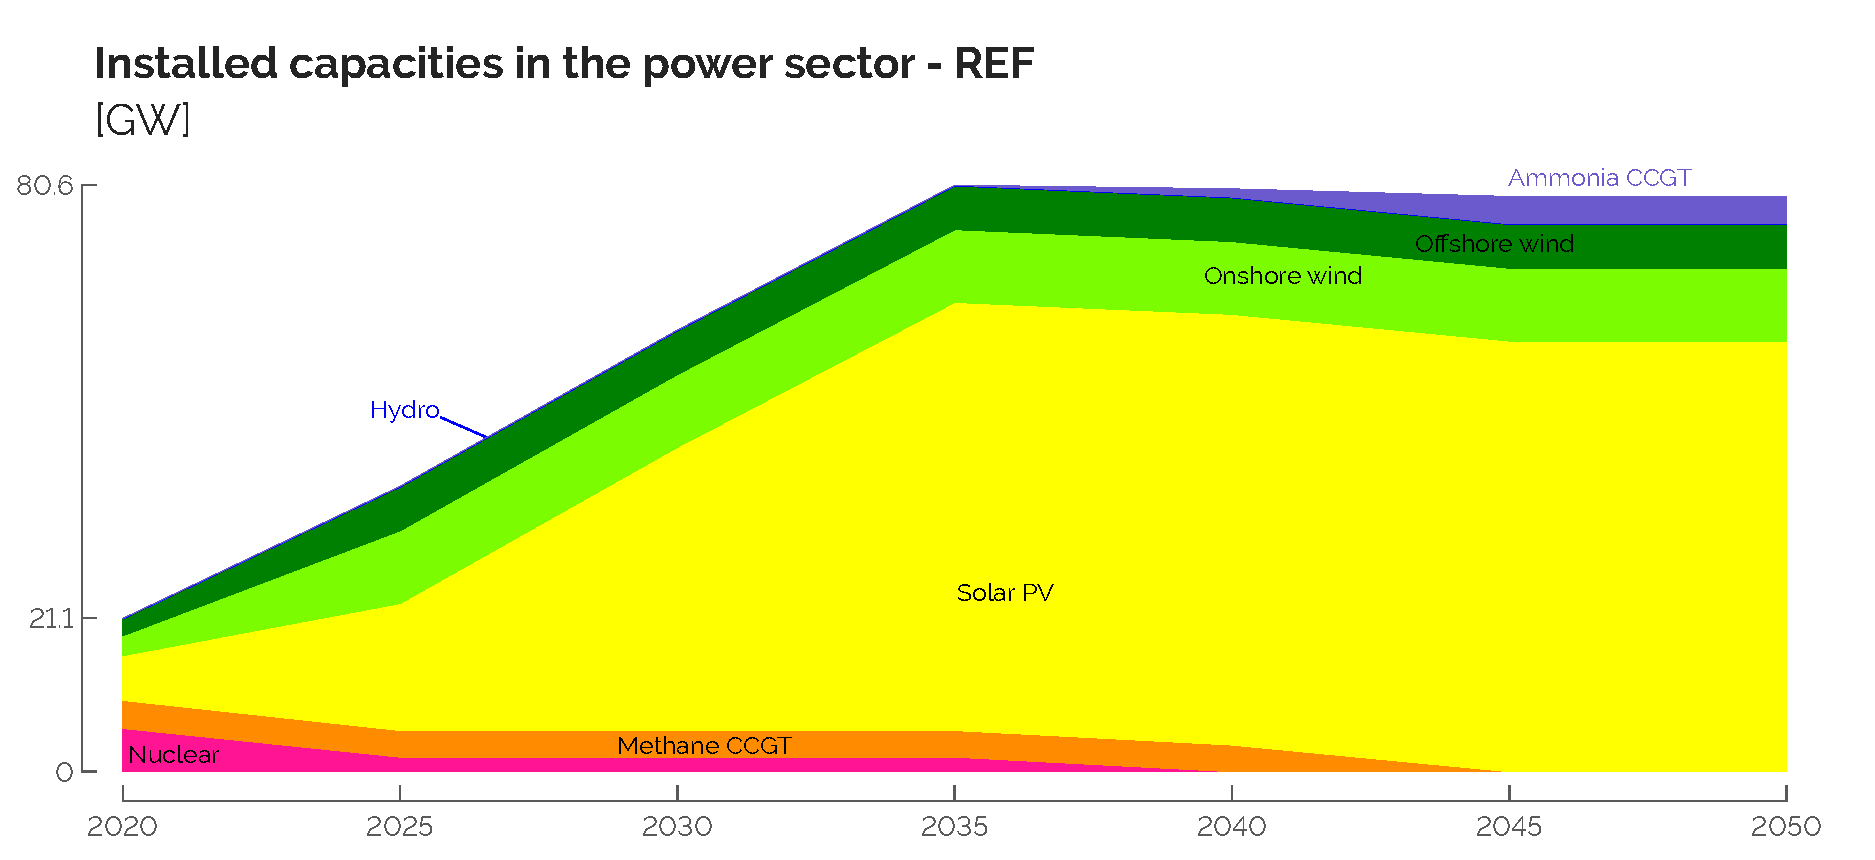
\includegraphics[width=0.8\textwidth]{Elec_Tech_Cap_REF.pdf}
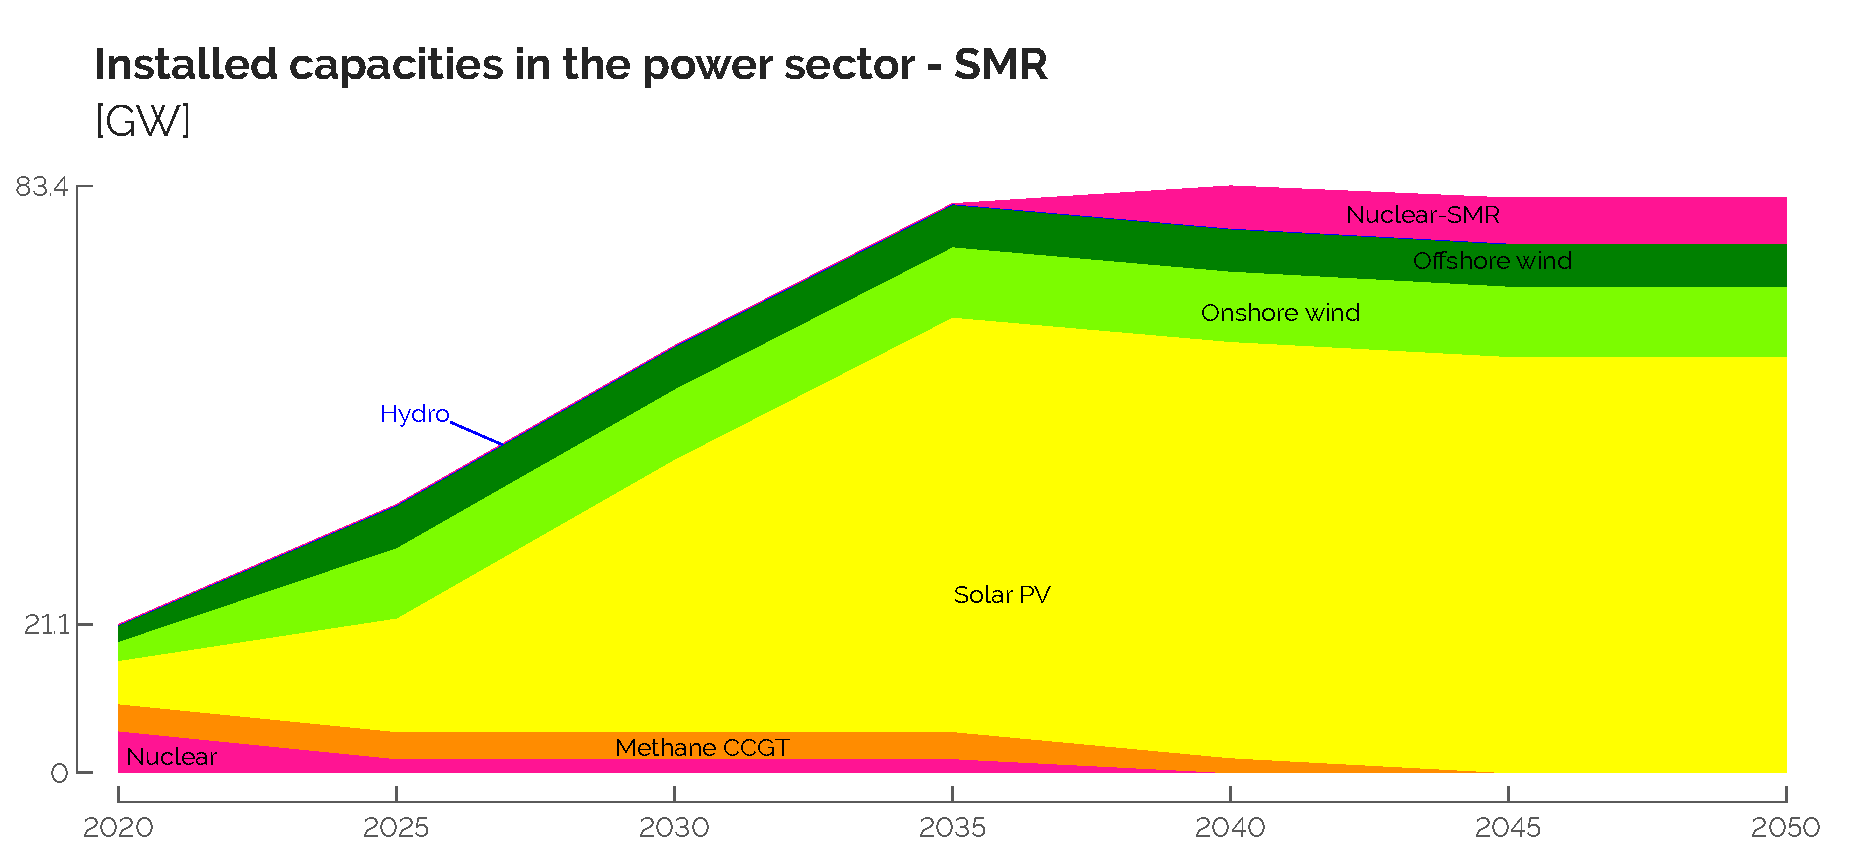
\includegraphics[width=0.8\textwidth]{Elec_Tech_Cap_SMR.pdf}
\caption{As soon as available (\ie 2040), \acrfull{SMR} is deployed to their maximum potential (\ie 6\,GW) to substitute more expensive flexible generation units (\ie gas and ammonia \gls{CCGT}).}
\label{fig:results_deter_tech_cap_elec}
\end{figure}

When assessing the electricity production-versus-consumption-balance (\Cref{fig:results_deter_layer_elec}), \gls{SMR}, as a cheaper, flexible and low-emitting power generation system, produces to its full capacity, given the 15\% maintenance off-time assumed in this work: 44.6\,TWh. By 2050, it represents 24.6\% of the total electricity production which is less than the current share of conventional nuclear in Belgium, 38.5\%. This resurgence of nuclear electricity occurs at the expense of other, although more efficient technologies: \gls{CCGT} and industrial \gls{CHP}. Besides the unchanged end-use-demand, we observe a slight increase of the electrification of the rest of the system: +9.4\% which corresponds to +5.8\,TWh, mostly consumed by electric heaters in industry (+48\%) to produce industrial high-temperature heat.

\begin{figure}[htbp!]
\centering
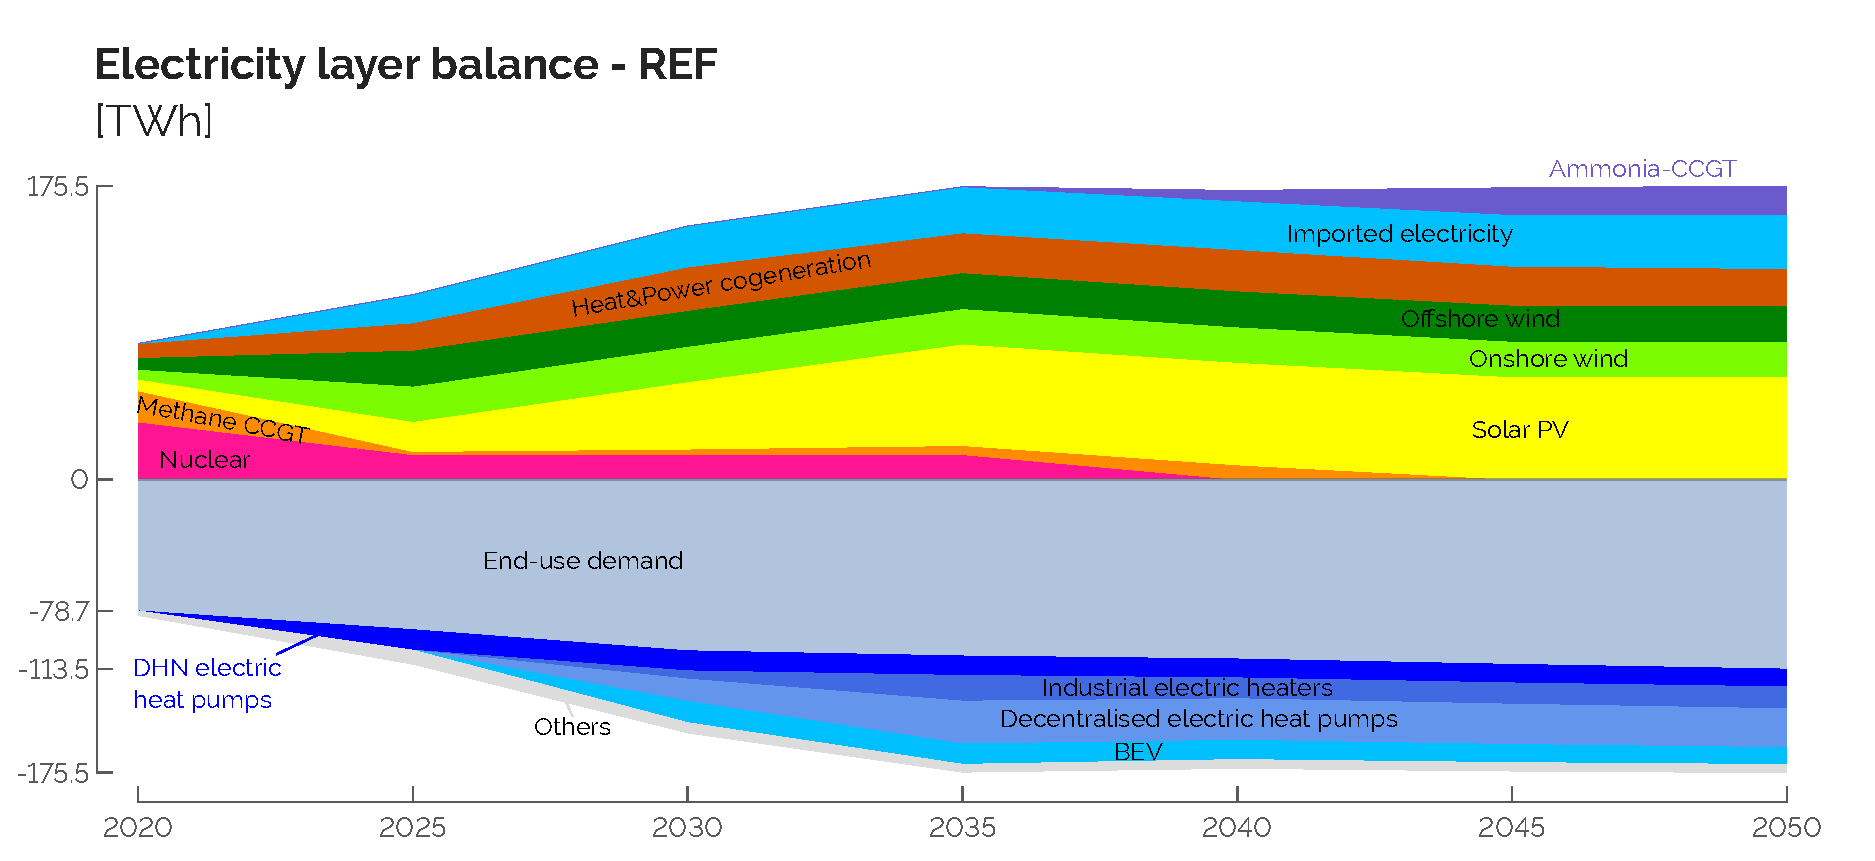
\includegraphics[width=0.8\textwidth]{Elec_Layer_REF.pdf}
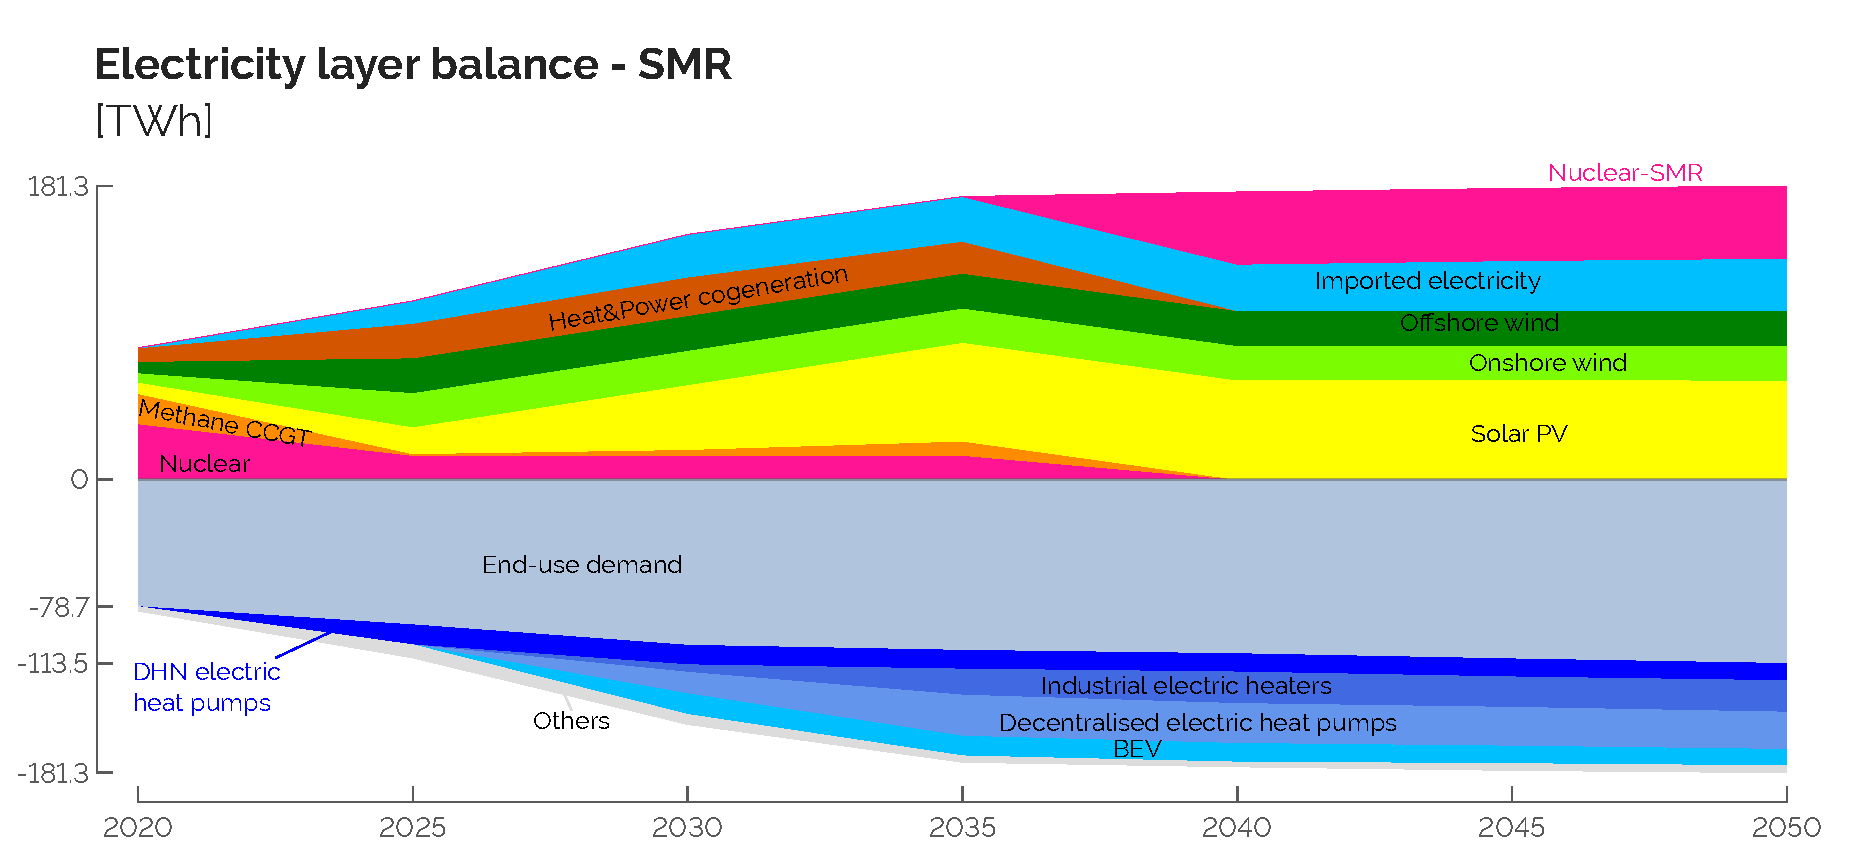
\includegraphics[width=0.8\textwidth]{Elec_Layer_SMR.pdf}
\caption{The production of electricity from \gls{SMR} substitutes more efficient technologies (\ie \gls{CCGT} and \gls{CHP}) and boosts the electrification of the rest of the system, mostly the industrial high-temperature heat sector.}
\label{fig:results_deter_layer_elec}
\end{figure}


\subsection{System-level impacts}
\label{subsec:atom_mol:results_deter_overall}
First of all, as far as the objective function (\ie the total transition cost) is concerned, \Cref{fig:results_deter_overall_emissions_sector} shows that the 6\,GW \gls{SMR} installed from 2040 allow reaching a 3.3\% (-36.9\,b€, $\sim$\,6\% of the Belgian GDP) cheaper overall transition. Interestingly, as the model can freely spend the constrained \ce{CO2}-budget over the transition, knowing ahead (\ie perfect foresight) that cheaper and low-emitting \gls{SMR} will be available in the future, cost-savings, that are more important after 2040, also occur before 2040. This is mostly due to the extended use of cheaper \gls{LFO} at the beginning of the transition to produce \gls{HVC}, that is then compensated by the deployment of \gls{SMR} (\Cref{fig:results_deter_overall_emissions_sector}). Then, the capital-intensive investments in \gls{SMR}, mostly recovered by the end of the transition as salvage value, are widely compensated by the smaller resource-related OPEX. This leads, at the end, aggregating the OPEX and the annualised CAPEX, to a system that is yearly 8.8\% less expensive by 2050.

\begin{figure}[htbp!]
\centering
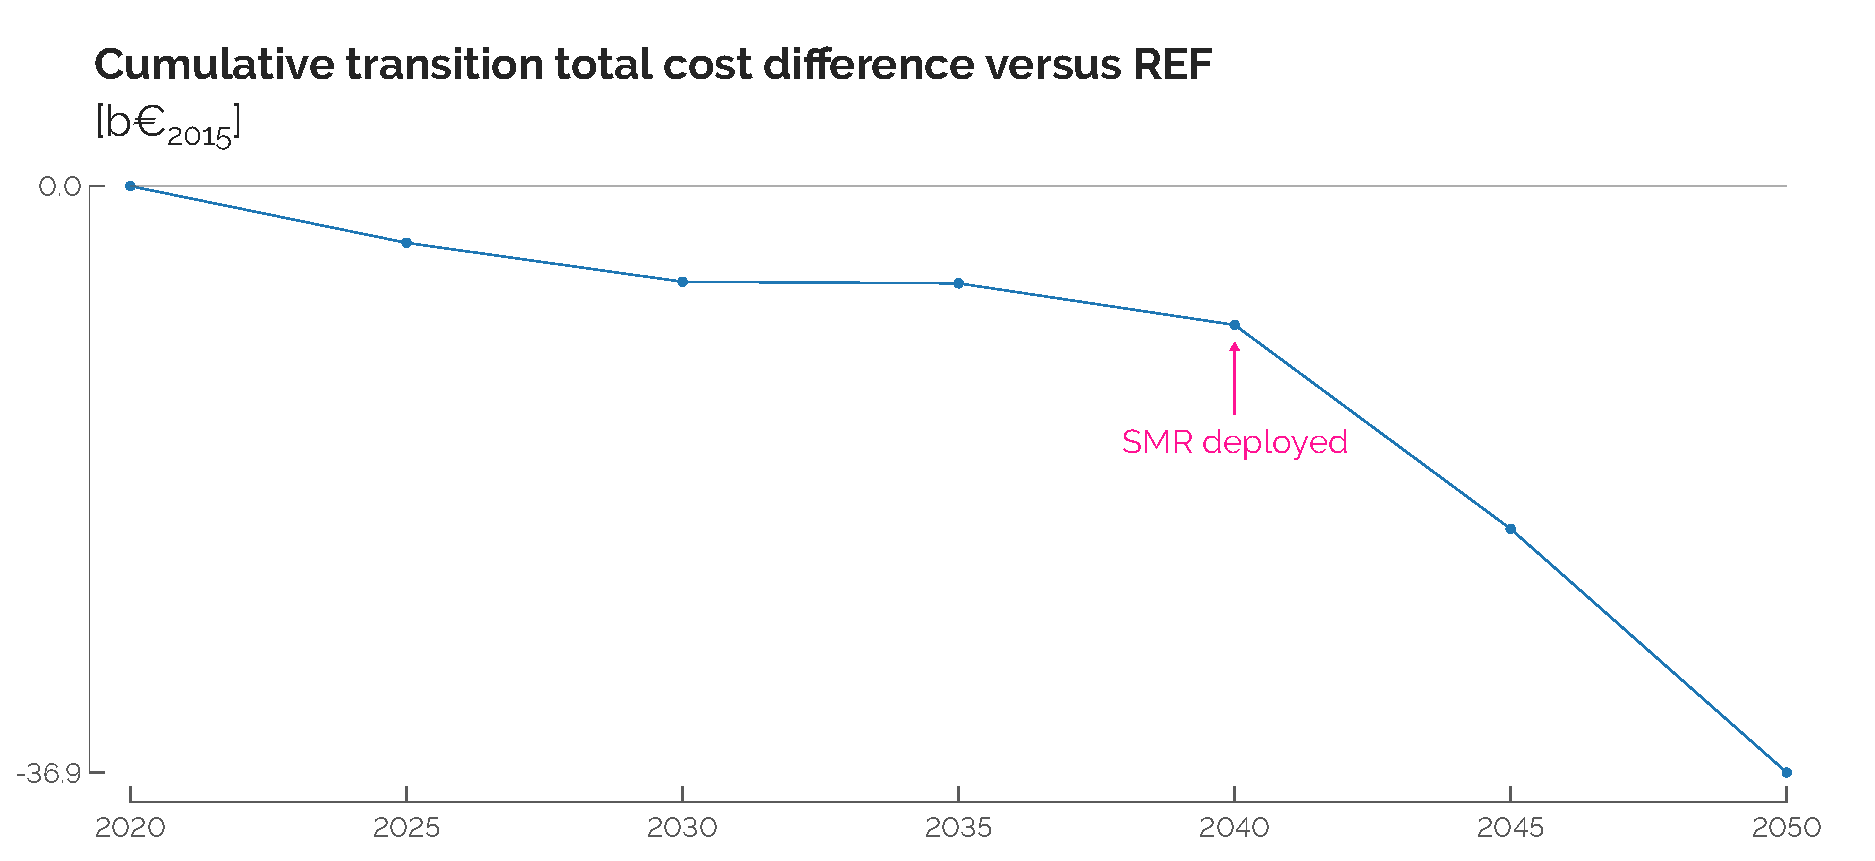
\includegraphics[width=0.8\textwidth]{Cum_total_cost_diff_REF.pdf}
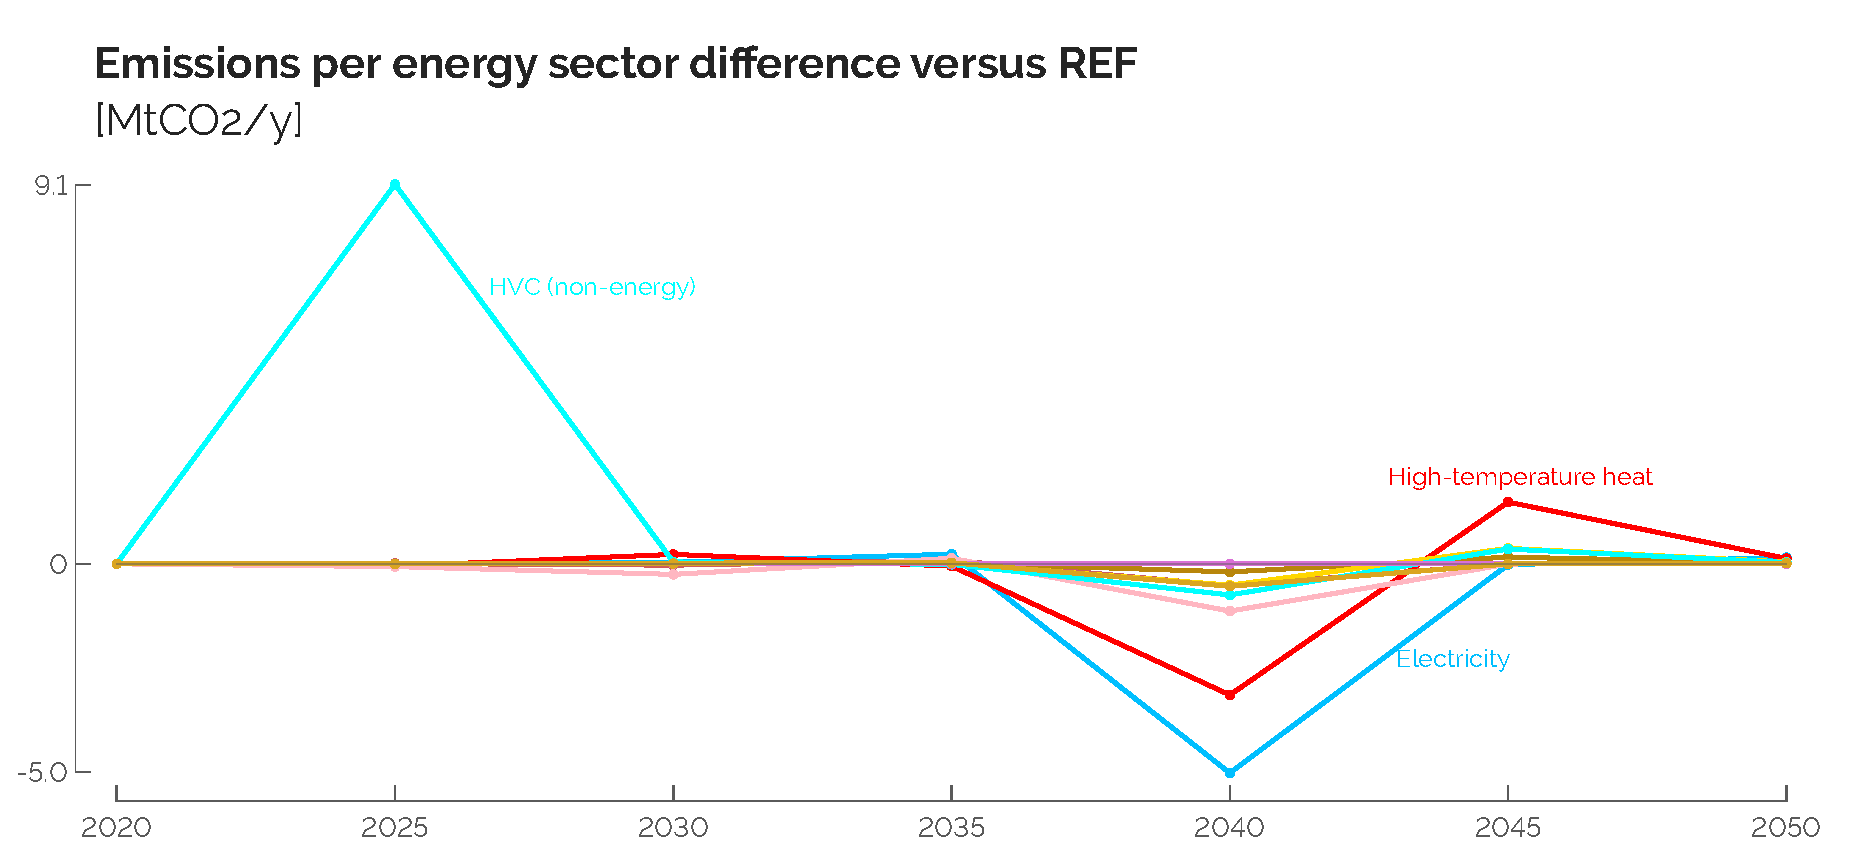
\includegraphics[width=0.8\textwidth]{GWP_per_sector_diff.pdf}
\caption{(Left) Cumulative transition cost difference between the SMR and the REF cases. Including \gls{SMR} ends up in a cheaper overall transition (\ie -3.3\%, -36.9\,b€). (Right) Emissions per energy sector differerence between the SMR and the REF cases. The deployment of \gls{SMR} from 2040 onward allows maintaining longer the use of \acrfull{LFO} for the production of \acrfull{HVC}.}
\label{fig:results_deter_overall_emissions_sector}
\end{figure}

Then, considering the primary energy mix shown in \Cref{fig:results_deter_energy_mix}, three phases in the transition can be identified. Before 2040, thanks to the perfect foresight approach, the model finds it more economical in 2025 to keep on using 33.2\,TWh of \gls{LFO} to produce \gls{HVC} through naphtha/LPG-cracking. In 2040, uranium-driven \gls{SMR} substitutes the electricity originally produced from industrial \gls{CHP} and \gls{CCGT} running respectively on fossil gas and renewable ammonia. Finally, from 2045 onward, the significant drop in the consumption of electrofuels comes from the same industrial \gls{CHP}. This is the illustration of the atom-molecules dilemma where the consumption of local renewables is, on its side, not much affected. In other words, \gls{SMR} competes with importing electrofuels while both support the integration of local solar and wind energies. Then, like the power sector, the SMR case ends up in a less efficient whole-energy system by 2050 at it consumes 47\,TWh (+12.7\%) primary energy more to supply an unchanged \gls{EUD}. Interestingly, in both cases, given the assumptions made on the \gls{GWP} of the resources (\ie $\mathit{gwp}_{\mathrm{op,electrofuels}}=0$\,kt$_{\ce{CO2},\text{eq}}$/GWh and $\mathit{gwp}_{\mathrm{op,uranium}}=0.004$\,kt$_{\ce{CO2},\text{eq}}$/GWh), the constraint on the \ce{CO2}-budget leads to ``carbon-neutrality'' by 2050\footnote{The model being constrained to keep on using all the waste that would keep on being locally produced, the system in 2050 reaches a $\sim 3.5\,Mt_{\ce{CO2},\text{eq}}$/year.}.

\begin{figure}[htbp!]
\centering
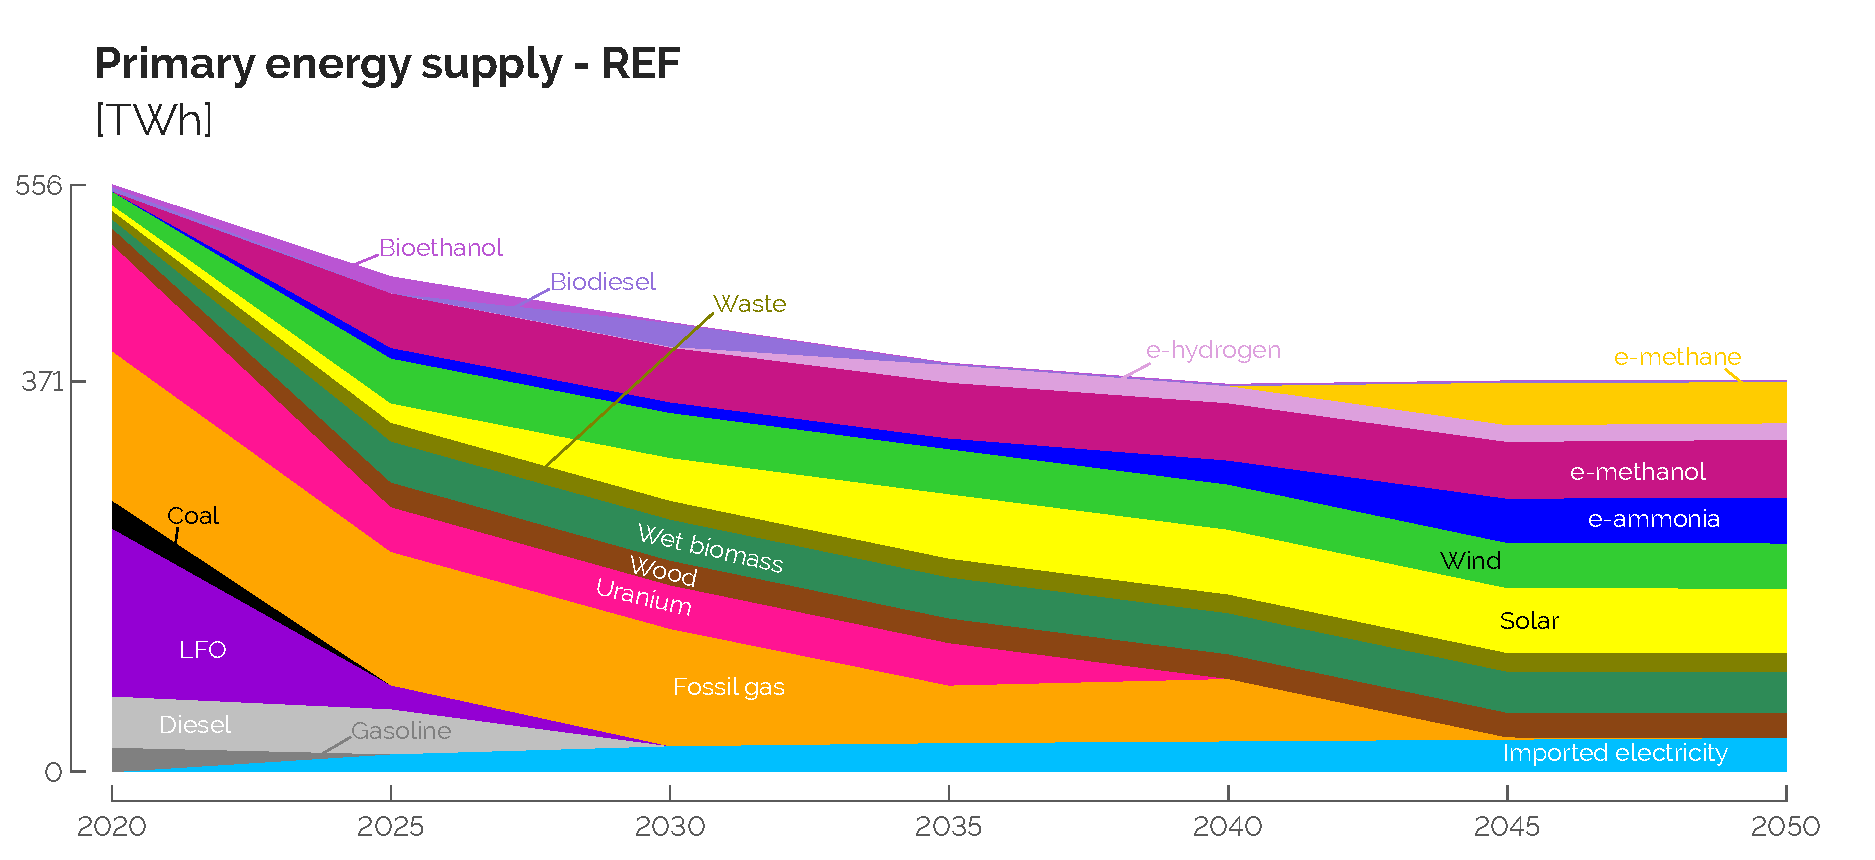
\includegraphics[width=0.8\textwidth]{Primary_mix_REF.pdf}
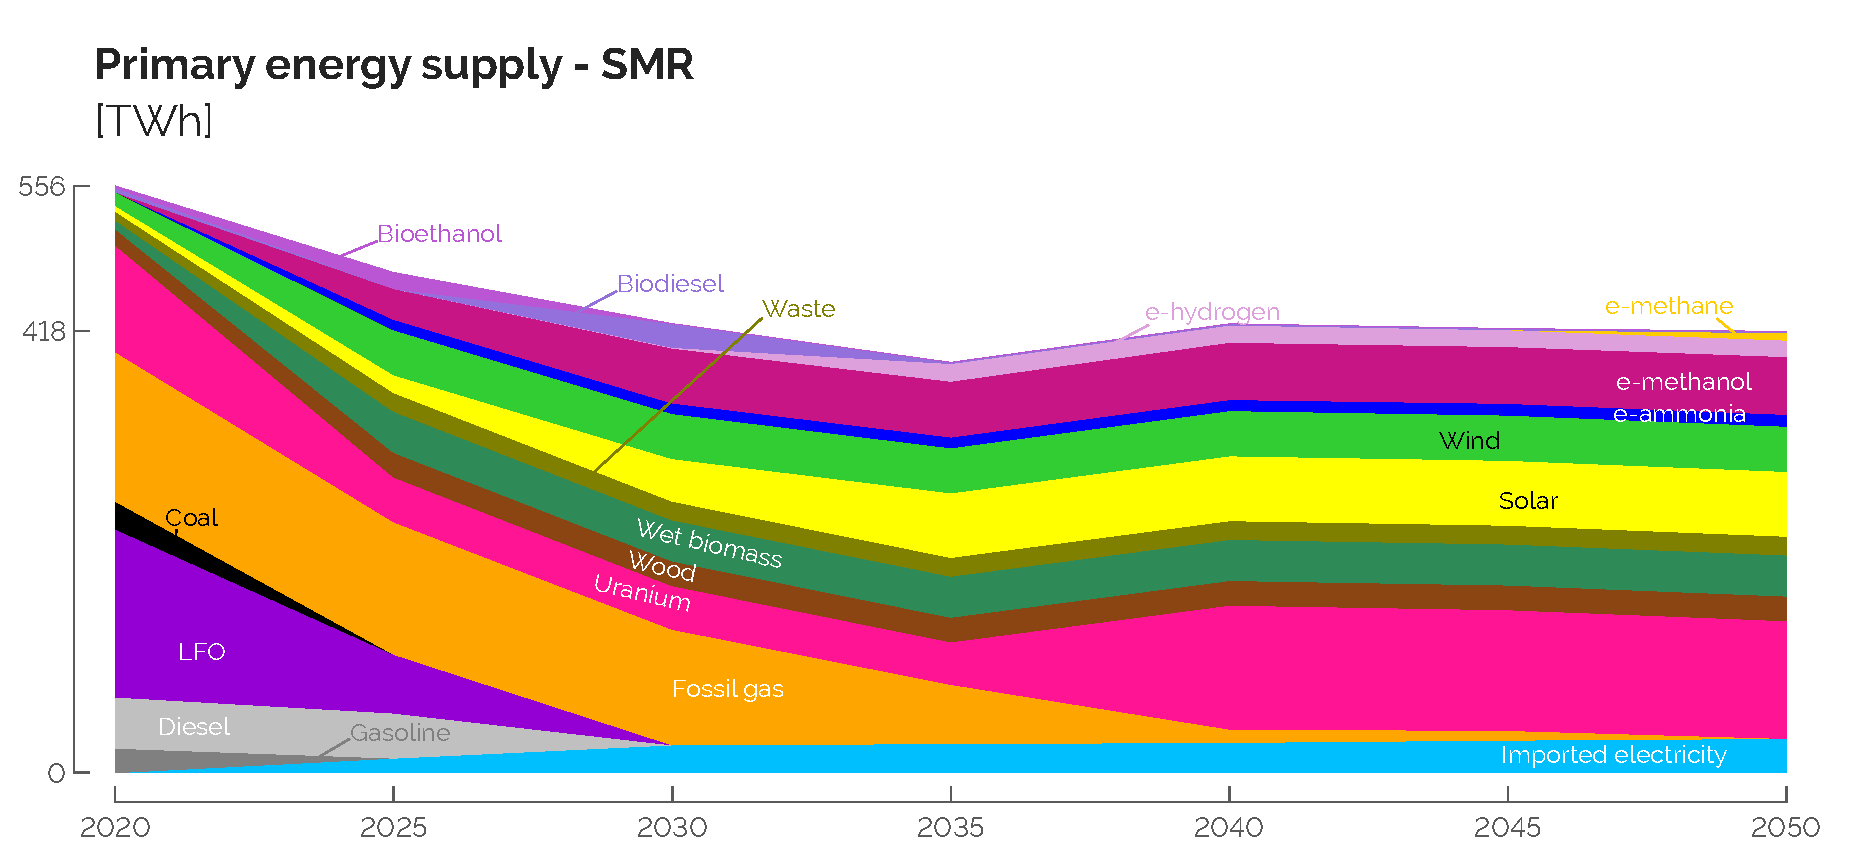
\includegraphics[width=0.8\textwidth]{Primary_mix_SMR.pdf}
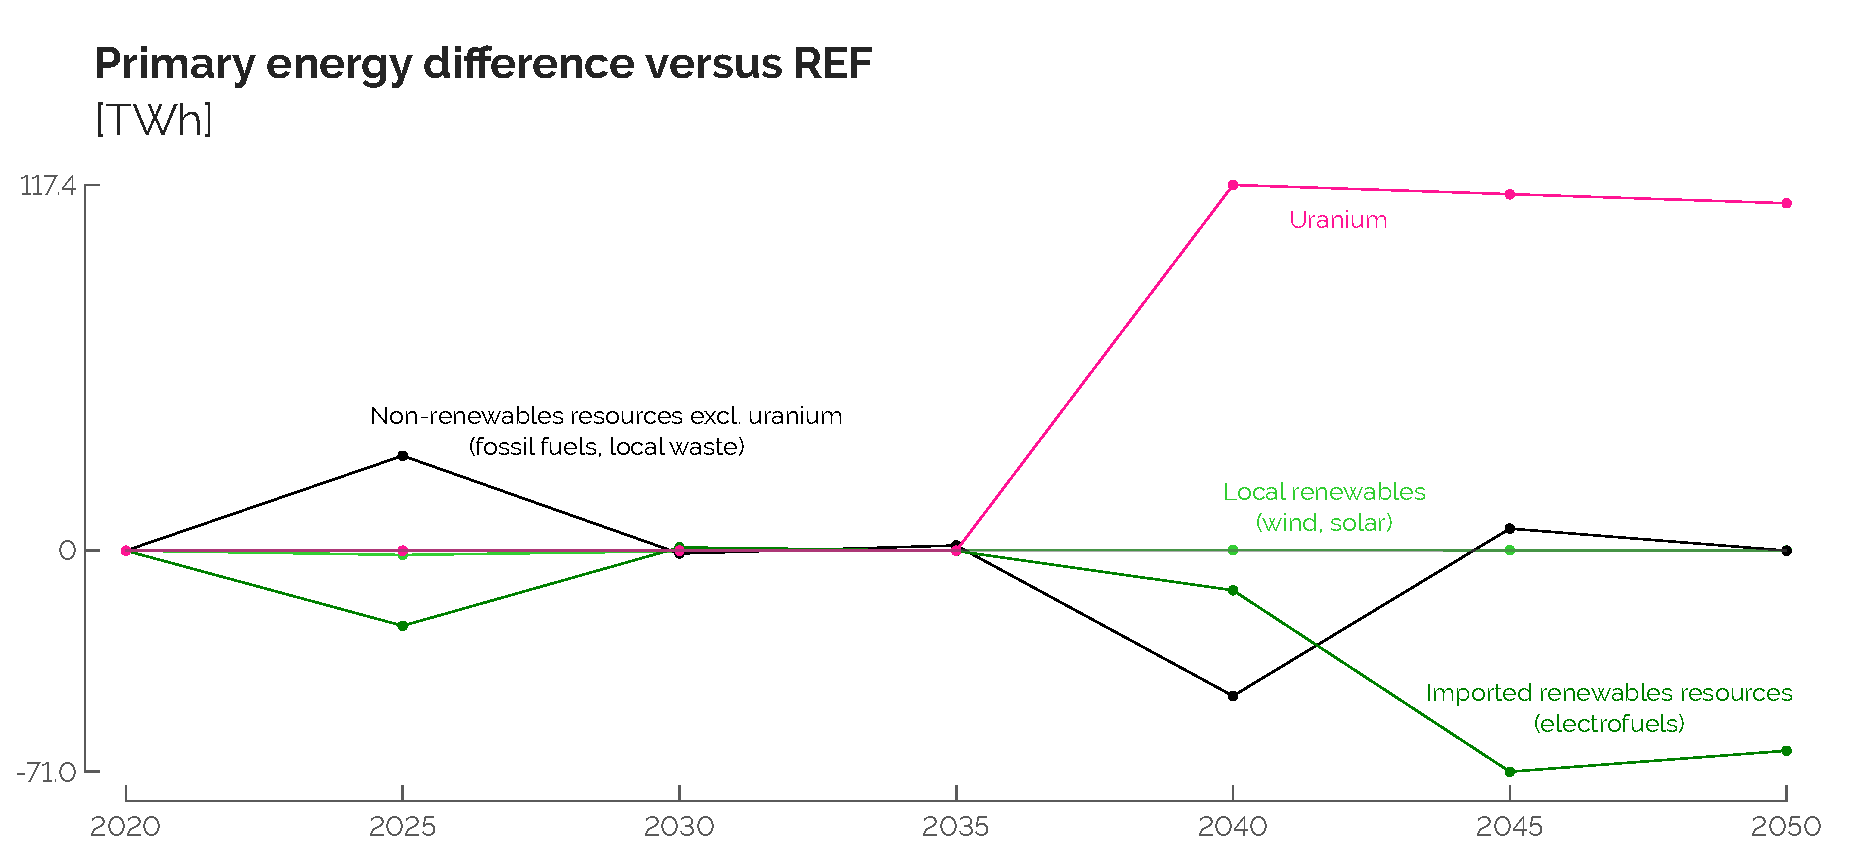
\includegraphics[width=0.8\textwidth]{Primary_mix_diff_uranium.pdf}
\caption{(Up) Primary energy mix over the transition for the REF and SMR cases. (Bottom) Difference of the mix between the two cases after aggregation per category. In Uranium, considered as a non-renewable resource in line with \citet{rixhon2021terminology}, is nevertheless dissociated from other non-renewable resources for the sake of clarity. The imported electricity is split between imported non-renewable and renewable resources assuming a linear decrease between the current share of renewables, \ie 37.41\% \cite{eurostat_share_re_elec}, and an assumed 100\%-renewable European electricity mix by 2050.}
\label{fig:results_deter_energy_mix}
\end{figure}

\subsection{Non-power sectors}
\label{subsec:atom_mol:results_deter_others}

Beyond the direct impact that \gls{SMR} has on the power sector, it is worth assessing the other sectors given the sector-coupling effect related to the whole-energy system optimisation \cite{contino2020whole}.\\

\myparagraph{High-temperature heat}\\

As aforementioned, the main impact of including \gls{SMR} from 2040 onward on the high-temperature heat sector is (i) its higher direct electrification and (ii) the reduction of overall more efficient heat-and-power co-generation in the benefit of single-output industrial boilers. On the one hand, in the REF case, industrial electric heaters are mainly used to absorb, instead of curtailing, the ``over-production" of the 59\,GW solar-PV when fully deployed, in the sunny days. With \gls{SMR}, by 2050, an additional 1.7\,GW (+13\%) of these heaters can rely on a more constant supply of defossilised electricity, consequently increasing their load factor and yearly production respectively by 31\% and 48\%. On the other hand, given the 44.6\,TWh of electricity produced by \gls{SMR}, cogeneration units are less relevant and, by 2050, 2.6\,GW industrial gas boilers completely substitute \gls{CHP} to produce 16.6\,TWh (\ie 23\%) of the total production of high-temperature heat.\\

\myparagraph{Low-temperature heat}\\

This sector is marginally impacted. In both cases, the major shift of supply from decentralised to centralised productions operates early in the transition, to hit the constraint that \gls{DHN} cannot supply more than 37\% of the \gls{LT}-heat production. Then, from a mix between oil (53\%), gas (43\%) and wood (4\%) boilers for the decentralised production of \gls{LT}-heat in 2020, the system progressively shifts towards electric \gls{HP} only. Similarly for the centralised production of \gls{LT}-heat, electric \gls{HP} remains the most efficient and economic option.\\

\myparagraph{Mobility}\\

The passenger mobility is not affected either as the electrification of the system is preferentially done in this sector with \gls{BEV} progressively substituting \gls{ICE} cars for the private sector. About the public mobility, trains and tramways supply their \textit{a priori} set maximum share, respectively, 50\% and 30\% complemented by \gls{CNG} buses substituting diesel-driven buses. Similarly, considering the freight transport, technology shifts (\ie from diesel to \gls{FC} trucks) or modal shares (\ie 53\%-47\% split between \gls{NG} and (bio)-diesel boats) are identical between the two cases.\\

\myparagraph{Non-energy demand}\\

The supply of ammonia (\ie from Haber-Bosch to direct import of renewable ammonia) and methanol (\ie import of renewable methanol) are unchanged between the two cases. However, as introduced previously, to produce \gls{HVC}, the full substitution of naphtha/LPG-cracking by \gls{MTO} is delayed as the emissions of the former are compensated by the later integration of \gls{SMR}.

\section{Uncertainty quantification on the cost, the atom and the molecules}
\label{sec:atom_mol:results_uq}
``\textit{It is difficult to make predictions, especially about the future.}" (Niels Bohr, foundational contributor to the understanding of atomic structure and quantum theory). Besides the deep understanding of the deterministic results, it is important to challenge these conclusions out-of-sample, accounting for the uncertainty of the parameters. After briefly assessing the \gls{GSA} on the objective function of the model, the total transition cost, this section investigates more deeply the atom-molecules dilemma. This time, the Sobol' indices are computed for import of renewable molecules and installed capacities of \gls{SMR}.

\subsection{Total transition cost}
\label{subsec:atom_mol:results_uq_cost}
Exhaustively listed in Appendix \ref{app:UQ_transition_cost}, \Cref{tab:UQ_short} gathers the most impacting parameters\footnote{Per \citet{Turati2017}, parameters are considered as ``impacting'' if their Sobol' index is above the threshold $=1/d$, $d$ being the total number of uncertain parameters after the pre-selection phase. In this case, $d=34$, and, consequently, the threshold is equal to 2.9\%.} on the total transition cost, highlighting the cost of purchasing electrofuels as well as the potentiality to install \gls{SMR} and its CAPEX. The former is the most impacting parameter whereas the two others have much lower influence on the variation of the total transition cost. Given the uncertainty characterisation presented in Section \ref{sec:cs:uncertainty}, there are 60\% chance that no \gls{SMR} could be installed. In other words, the variation of the parameter $f_{\mathrm{max,SMR}}$ has zero impact on the variation of the total transition cost in 60\% of the samples. Then, in perspective with the local sensitivity analysis of Section \ref{sec:atom_mol:results_deter}, the 3.3\% reduction has been observed when \gls{SMR} is installed from 2040 onward. This represents only 10\% of the samples. Moreover, given its characteristics detailed in \Cref{tab:SMR_features}, mostly its cheap and low-emitting fuel (\ie uranium) and the long lifetime leading to lower annualised CAPEX and higher salvage value, this explains why \gls{SMR} has this lower impact. On the contrary, more expensive renewable electrofuels are always imported, to a smaller or larger extent depending on the sample. For instance, in the REF case (Section \ref{subsec:atom_mol:results_deter_overall}), the imported electrofuels represent, by 2050, 152.9\,TWh (\ie 41\% of the primary energy mix) with an average 93€/MWh cost of purchasing and, over the entire transition, a 273\,b€ cumulative OPEX (\ie 25\% of the total transition cost).

\begin{table}[htbp!]
\caption{Total Sobol' indices of the uncertain parameters over the total transition cost. Where the cost of purchasing electrofuels is the top-1 parameter, \gls{SMR}-related parameters have a negligigble impact on this cost.}
\label{tab:UQ_short}
\centering
\begin{tabular}{l c c}
\toprule
\textbf{Parameter}  & \textbf{Ranking} & \textbf{Sobol' index} \\	
\midrule
\textbf{Purchase electrofuels} & 1 & 46.8\% \\
Industry EUD & 2 & 23.2\% \\
Interest rate & 3 & 12.0\% \\
Purchase fossil fuels  & 4 & 5.7\% \\
$\vdots$ & $\vdots$ & $\vdots$\\
\textbf{Potential capacity \gls{SMR}} & 11 & 0.9\% \\
$\vdots$ & $\vdots$ & $\vdots$\\
\textbf{CAPEX \gls{SMR}} & 33 & $<$0.1\% \\
\bottomrule							

\end{tabular}
\end{table}

Given the relatively wide uncertainty range (\ie up to [-30.8\%; +24.0\%] by 2050) and, above all, the major share among the total demand, between 53\% and 60\%, the industrial \gls{EUD} is the second most impacting parameter. Then, as the driving factor for the annualisation and the salvage value of the assets, the interest rate has a 12\% Sobol' index\footnote{It is important to note here that the model considers an overall interest rate for the entire system (\ie 1.5\% as a nominal value). In practice, the interest rate would vary depending on the technology investment risk. This variation would have, for instance, a major impact on the \gls{LCOE} of technologies like nuclear power plants \cite{world_nuclear_asso}, given the important capital needs and long time horizons \cite{IEA_Nuclear_2022}.}. Finally, similarly to electrofuels, the cost of purchasing fossil fuels is also to consider in the perspective to reduce the uncertainty over the total transition cost. However, due to the ambitious \ce{CO2}-budget, phasing out of fossil fuels is urgent and makes their uncertain impact smaller than their renewable alternatives.

\Cref{fig:UQ_PDF_total_transition_cost} shows the \gls{PDF} of the total transition cost given the 1260 samples. Stretching between 660\,b€ and 2050\,b€, the mean, the median and the nominal value (\ie REF case) are close to each other, respectively 1180\,b€, 1160\,b€ and 1080\,b€. Similarly to the analysis carried out by \citet{coppitters2023optimizing}, one observes here that the distribution is right-skewed. It could then be qualified as ``fragile" as the top 50\% of the samples cover a bigger range (\ie between 1160 and 2050) than the bottom 50\% of the samples (\ie between 660 and 1160). In other words, the bad scenarios, resulting in a total transition cost higher than the median, have a bigger effect on this cost.

\begin{figure}[htbp!]
\centering
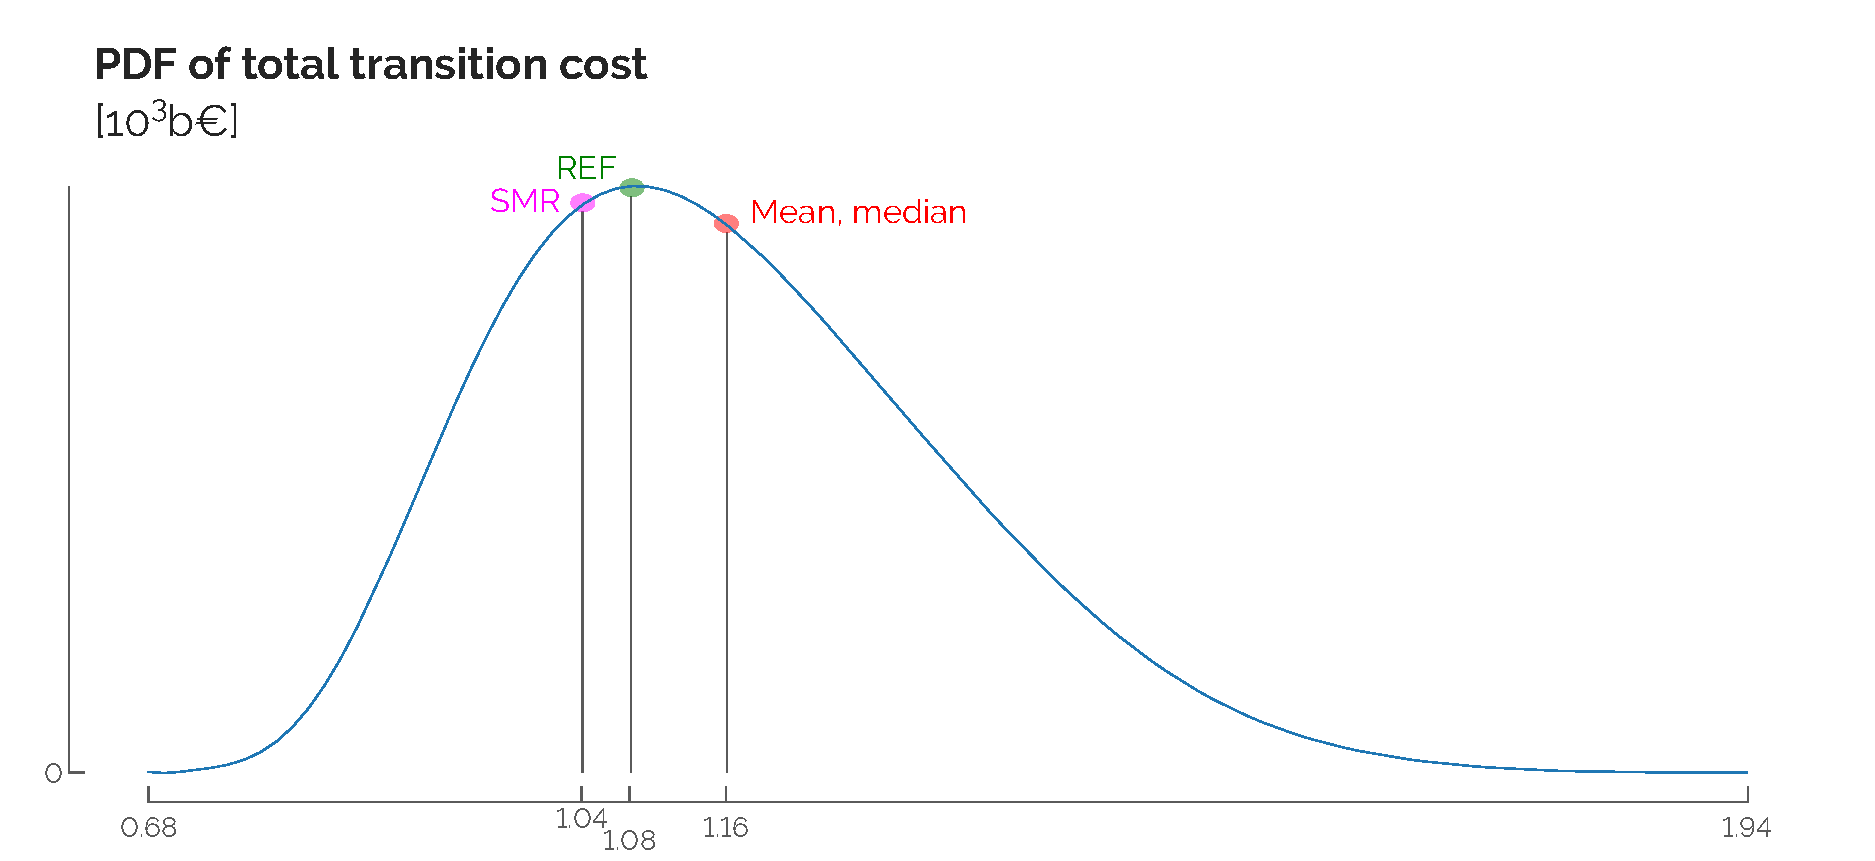
\includegraphics[width=0.8\textwidth]{UQ_PDF_total_transition_cost.pdf}
\caption{\acrfull{PDF} of the total transition cost. The mean, $\mu=1.18\cdot10^3$\,b€, is slightly higher than the median ($P_{50}=1.16\cdot10^3$\,b€) and the nominal cases cost, $1.08\cdot10^3$\,b€ and $1.04\cdot10^3$\,b€ respectively for the REF and SMR cases. Also, with a standard deviation, $\sigma=197$\,b€, a 95\%-confidence interval would be about [0.8; 1.6]$\cdot10^3$\,b€.}
\label{fig:UQ_PDF_total_transition_cost}
\end{figure}

\subsection{Atom and molecules}
\label{subsec:atom_mol:results_atom_mol}
The samples used to carry out the \gls{GSA} on the total transition cost, also provide the distribution of other outputs of the model. Among them, \Cref{fig:results_uq_electrofuels} shows the evolution of the import of renewable electrofuels over the transition.

As the general trends are increasing, discrepancies exist between the different energy carriers. E-methane, as the renewable alternative to fossil natural gas, substitutes it, sometimes at a very early stage of the transition, 2025, and to a somehow unrealistically large extent, 163\,TWh, which is more than 6\% more than the total import of electrofuels in the REF case. The necessity to import this molecule is progressive through the transition to supply mostly industrial \gls{CHP} and boilers. 

E-hydrogen becomes rapidly the main stream of hydrogen in the system, on top of steam-methane-reforming or electrolysis, to reach a median and a maximum values of, respectively 13.0\,TWh and 42.1\,TWh in 2050. Hydrogen is more frequently used in the mobility sector. Like in the REF case, fuel cell trucks are often the first option but, in some outlying cases, fuel cell cars and buses appear to completely substitute respectively \gls{BEV} cars and \gls{CNG} buses by 2050. Moreover, some samples lead to local production of methanol via the methanolation process, to produce up to 17.8\,TWh of methanol (\ie 33\% of the total supply of methanol of the nominal REF and SMR cases). 

Then, the imported e-ammonia, becoming rapidly cost-competitive against its fossil alternative (\Cref{fig:cs_resources_cost}), quickly substitutes it and the Haber-Bosch process. Where the initial purpose of ammonia is to satisfy a relatively limited \acrfull{NED} (\ie 10 $\pm$ 3\,TWh by 2050), the variation of its import is mostly due to the higher or lower need for ammonia-\gls{CCGT} as a flexible option to produce electricity. From 2035, out of the four considered electrofuels, the imported e-ammonia is the one exhibiting the largest uncertainty with, for instance, an interquartile range (IQR)\footnote{The interquartile range is the difference between the third quartile ($Q3$ or $P_{75}$) and the first ($Q1$ or $P_{25}$). It is an indicator of statistical dispersion around the median, $Q2$ or $P_{50}$.} of about 50\,TWh. In some extreme cases, e-ammonia is the most imported molecules, \ie up to 216\,TWh or 58\% of the total primary mix in the REF case in 2050. 

Likewise, e-methanol early becomes the selected option to supply methanol even though alternatives like biomass-to-methanol or synthetic methanolation exist in some outlying cases. Given its lower \gls{NED} (\ie 1.5$\pm$0.5\,TWh$_{\text{NED,methanol}}$ by 2050), the variation of imported e-methanol is almost exclusively due to its role in the industrial production of \gls{HVC}, \ie 78\% of the total \gls{NED}, through the \acrfull{MTO} process. In some rare samples, methanol is also used to supply the freight transport sector via boats or trucks.

Appendix \ref{app:UQ_electrofuels} gives a more detailed information. On the one hand, it compares the statistics (\ie quartiles and median) with the quantity of imported electrofuels in the REF and SMR cases. On the other hand, this appendix shows the distributions of the different sources of supply and consumption of gas, hydrogen, ammonia and methanol.

\begin{figure}[htbp!]
\centering
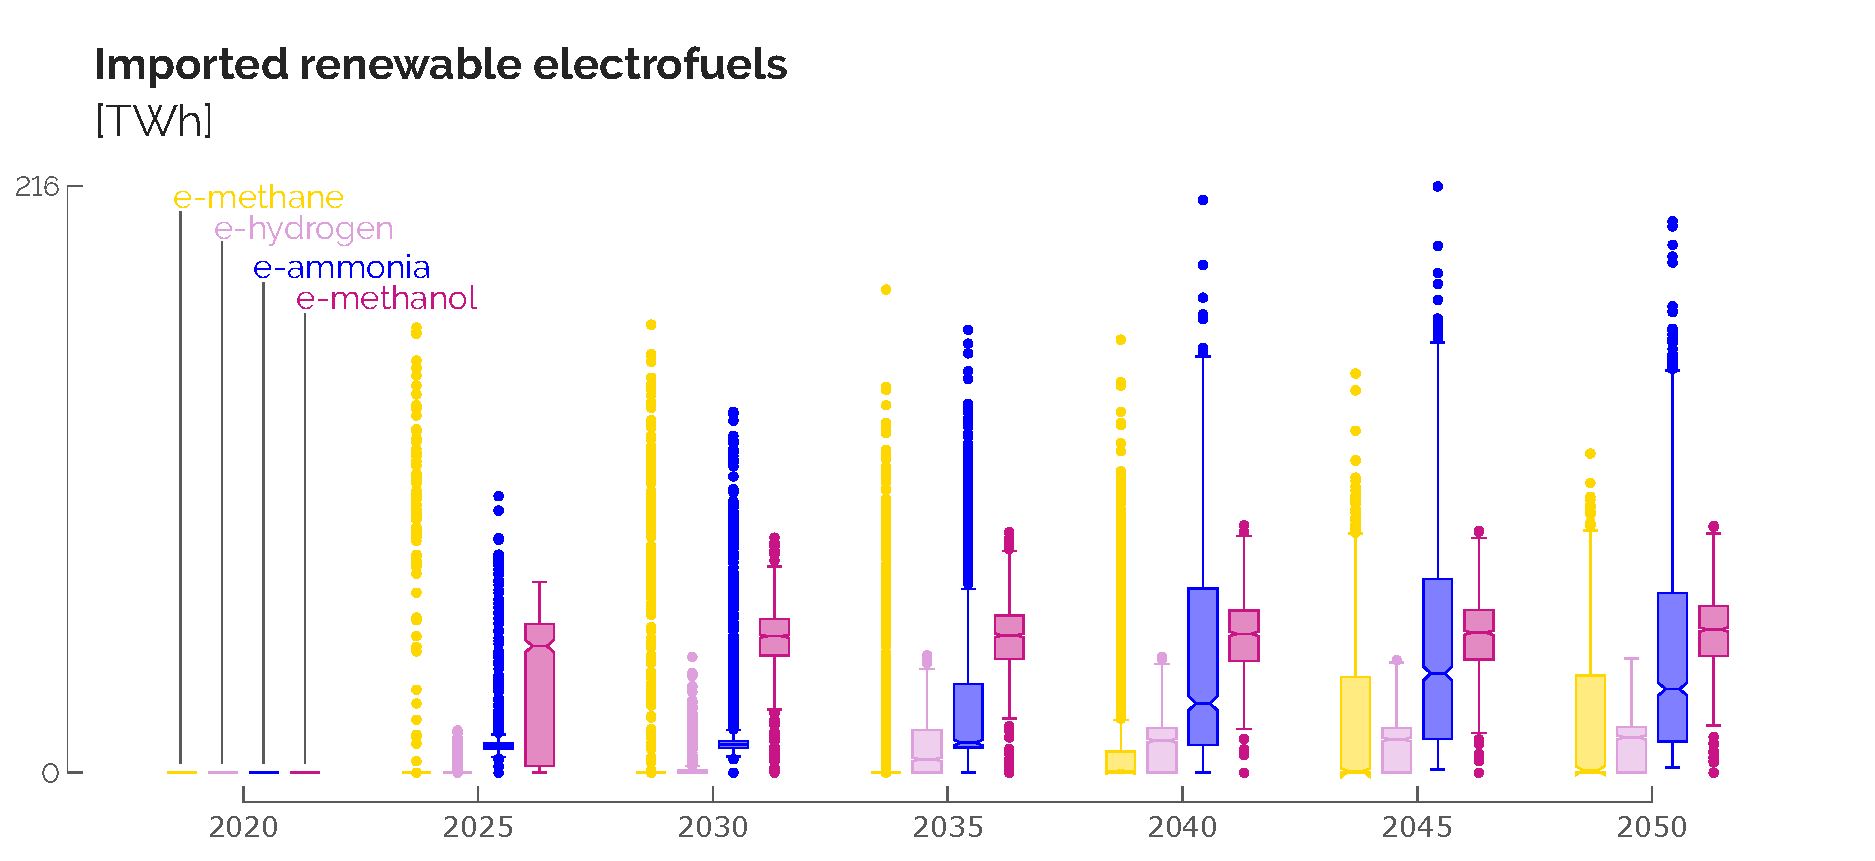
\includegraphics[width=0.7\textwidth]{UQ_Electrofuels.pdf}
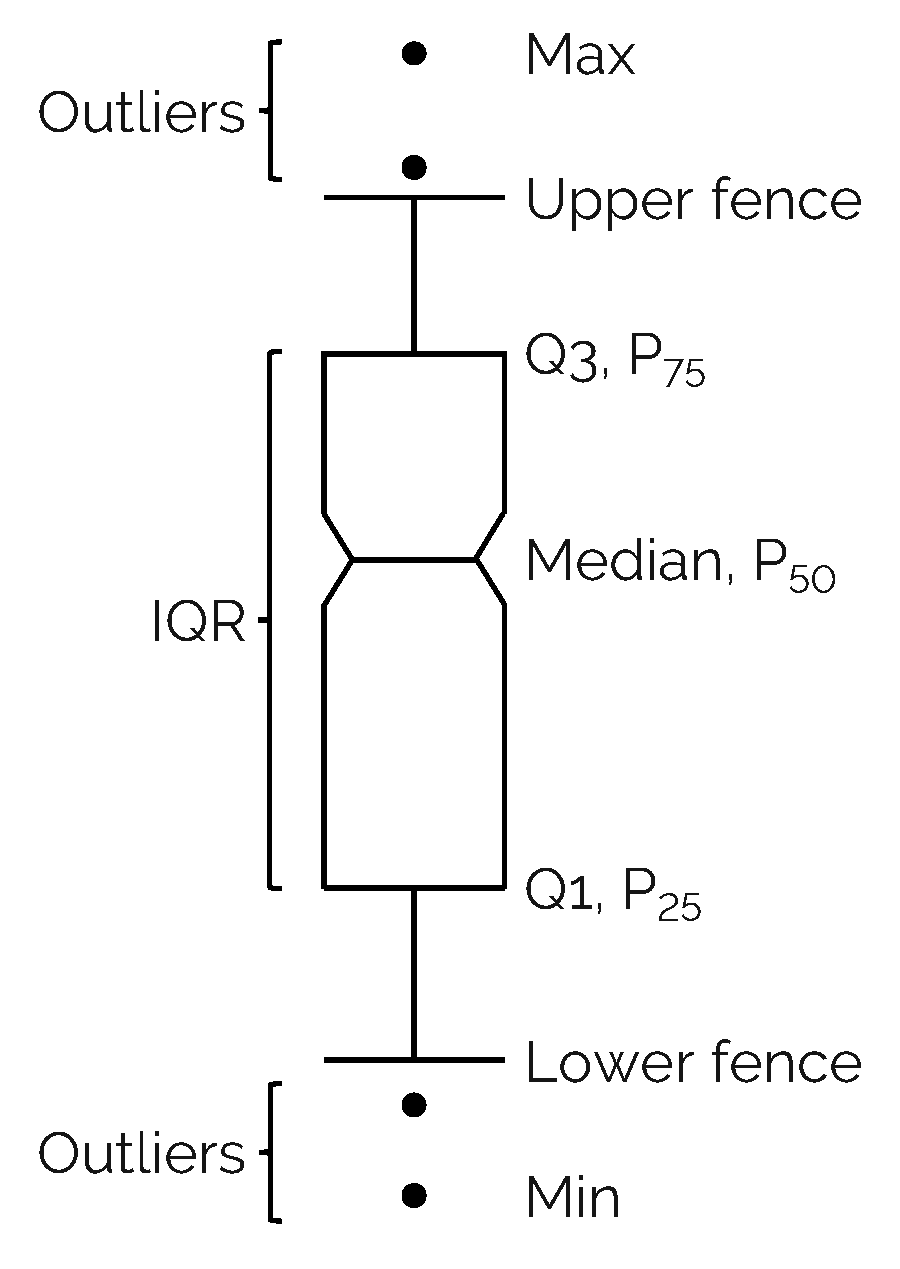
\includegraphics[height=4cm]{Schematic_boxplot.pdf}
\caption{Distribution of the imported renewable electrofuels over the transition. Starting from no electrofuel in 2020, their respective import rises progressively along the transition (\ie increasing median) at different growth rates and with different ranges of values. Observations being either 1.5 times the interquartile range (IQR) less than the first quartile (Q1) or 1.5 times the interquartile range greater than the third quartile (Q3) are defined as outliers.}
\label{fig:results_uq_electrofuels}
\end{figure}

After investigating the distribution of imports of electrofuels over the transition, this part assesses the space of uncertainties, like \citet{pickering2022diversity} who investigated the space of feasibility to reach carbon neutrality in Europe. Figures \ref{fig:results_uq_samples_A} and \ref{fig:results_uq_samples_B} give the trend lines of the key parameters for these imports in 2050\footnote{The authors picked this specific year as it is the one where electrofuels, if imported, are imported in the largest amount, in general, compared to the other years of the transiton.}, as well the installed capacities of \gls{SMR}. Next to the name of a parameter, one can read its Sobol' index versus the output of interest\footnote{For these outputs of interest, different from the total transition cost, the \gls{LOO} error is generally higher than the threshold of \SI{1}{\%} defined in Section \ref{subsec:pce}. Consequently, the Sobol' indices are less accurate but already allow a fair relative comparison between the different parameters.}. Box plots also point out the distribution of this output for the extreme low or high values of some parameters.

As aforementioned, the industrial \gls{EUD} impacts the most the import of e-methane. This parameter directly dictates the demand of industrial high-temperature heat for which industrial gas \gls{CHP}, and industrial gas boilers to a lower extent, represent, on average over all the samples, respectively 25.6\% and 6.1\% of the total production. Then, considering the smaller-impact parameters, we notice that \gls{SMR} plays a non-negligible role. Indeed, if deployed, \gls{SMR} produces abundant low-emitting electricity for industrial electric heaters that substitute, even completely in some cases, gas alternatives. This confirms the observation made in Section \ref{subsec:atom_mol:results_deter_others}. Highly available local biomass also leads to smaller import of e-methane to supply bio-hydrolysis and produce methane-equivalent gas. Finally, and surprisingly, costs of purchasing electrofuels and fossil fuels have a positive and negative correlation with the amount of e-methane, respectively. In other words, by 2050, more expensive electrofuels induce to more e-methane import and \textit{vice versa} for the fossil fuels. Given the techno-economic optimum sought by EnergyScope, if electrofuels are more expensive, the system will, overall, import less of them, especially e-ammonia, mainly used by \gls{CCGT}. Subject to the \ce{CO2}-budget for the transition, the system goes towards more efficient technologies, like industrial methane-\gls{CHP} to substitute e-ammonia-\gls{CCGT} in the production of electricity. First running on fossil natural gas, these \gls{CHP} consume more e-methane by 2050. In the contrary, if electrofuels are cheaper, there is more import of them, and especially of e-ammonia. This leaves room for more emitting and cheaper resources to be used while respecting the \ce{CO2}-budget, \ie coal in industrial boilers that produce, in these cases, on average 24\% of the high-temperature (HT) heat in 2050. In these cases, the use of coal in 2050 highlights that, with a sharper decrease of the emissions at early stages in the transition, the models finds a solution including highly-emitting resources (\eg coal) while respecting the \ce{CO2}-budget. Consequently, there is smaller investment in methane \gls{CHP}, and consequently import of e-methane as more abundant renewable electricity is produced via e-ammonia-\gls{CCGT} and more HT-heat is supplied by industrial coal boilers. Even though we might expect that no more coal will be consumed in Belgium by 2050, the model still has the opportunity to use it if the \ce{CO2}-budget allows it. About the cost of purchasing fossil fuels, the parameter has mainly an impact on the import of fossil \gls{NG} as the most versatile energy carrier in the whole-energy system. If \gls{NG} is more expensive, the system will import less of it. Subsequently, the investments in methane-\gls{CHP} and boilers are more limited. This ends up in smaller need for e-methane by 2050.

In relation to e-hydrogen, the sensitivity analysis highlights its dependence on various driving parameters, particularly those linked to the transport sector. As depicted in \Cref{fig:results_uq_prod_cons} in Appendix \ref{app:UQ_electrofuels}, the utilisation of e-hydrogen is most prevalent in \gls{FC} trucks, followed by \gls{FC} cars and buses to a lesser extent. The adoption of fuel cell engines in trucks contributes, on average, to 63.5\% of the total road freight transport, thereby affecting the level of e-hydrogen imports. Consequently, the smaller is the CAPEX of fuel cell engines, the more the system imports e-hydrogen. Similarly, the cost of purchasing electrofuels influences e-hydrogen imports. Subsequently, the cost of purchasing biofuels emerges as the third most influential parameter. Indeed, biodiesel trucks are the mostly picked alternative to \gls{FC} trucks to provide, on average, 27.6\% of the total. Additionally, \gls{CNG} buses are preferred in public road transport (34.9\%), followed by \gls{FC} buses (11.2\%) competing with biodiesel and hybrid biodiesel buses, accounting for 27.8\% and 26.1\%, respectively. Finally, the last noticeable parameter at stake is the CAPEX of electric vehicles. In competition with \gls{BEV} that stand for 83.4\% on average of the private mobility sector, the cheaper these cars are, the more cost-competitive are these vehicles, and vice versa, versus \gls{FC} cars (\ie 13.7\% of the total passenger mobility, on average).

As already pointed out in Section \ref{subsec:atom_mol:results_deter_power_sector}, the installation of \gls{SMR} drastically reduces the import of e-ammonia. As ammonia \gls{CCGT} is the biggest consumer of ammonia by the end of the transition, low-emitting and cheap electricity flexibly produced by \gls{SMR} substitutes the \gls{CCGT}. With a higher cost of purchasing electrofuels, this import of e-ammonia drops down to 2.0\,TWh, 95.4\% less than in the REF case. Then, with a 12\%-Sobol' index, the cost of purchasing electricity from abroad, considered as renewable by 2050 and, therefore, a direct competitor to e-ammonia \gls{CCGT}, also affects the need of this molecule, especially when this cost is low.

The conclusions are more straightforward for the import of e-methanol and the installed capacity of \gls{SMR}. For the former, industrial \gls{EUD} is, by far (\ie 79\% Sobol' index), the key factor. Due to its own \gls{NED} but, above all, since it is the low-emitting alternative picked by the model to supply the significant \gls{NED} of \gls{HVC}, the lower this demand, the lower the need to import e-methanol, and vice versa. For the latter, it is the availability of the technology that drives its installation. Not shown here but all the samples of the \gls{GSA} highlight that \gls{SMR} is installed to its maximum capacity, \ie 6\,GW, as soon as possible. In other words, the only parameter ``Potential capacity \gls{SMR}'' dictates the installation of this technology\footnote{In practice, we observe that as soon as this parameter is equal or higher than 0.9, 0.8 and 0.6, 6\,GW \gls{SMR} is installed from 2040, 2045 and 2050, respectively.}. Surprisingly, the [-40\%; +44\%]  variation of its CAPEX has a negligible impact, with a Sobol' index of 0.9\%.

\begin{figure}[htbp!]
\centering
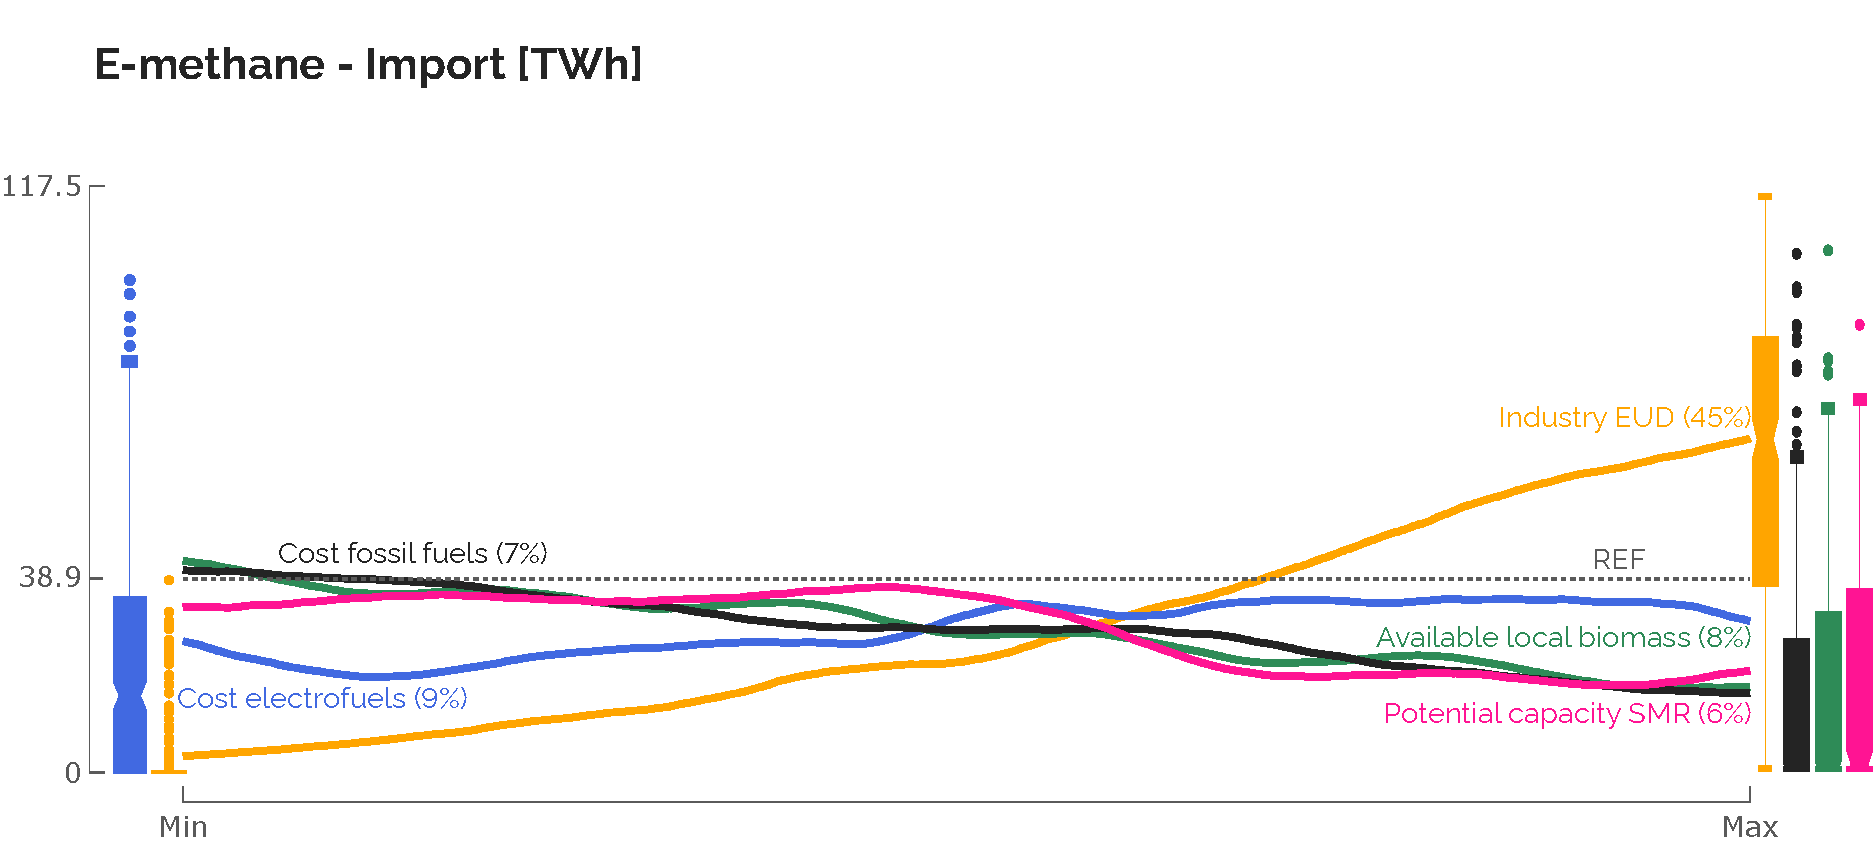
\includegraphics[width=0.8\textwidth]{UQ_Gas_samples_2.pdf}
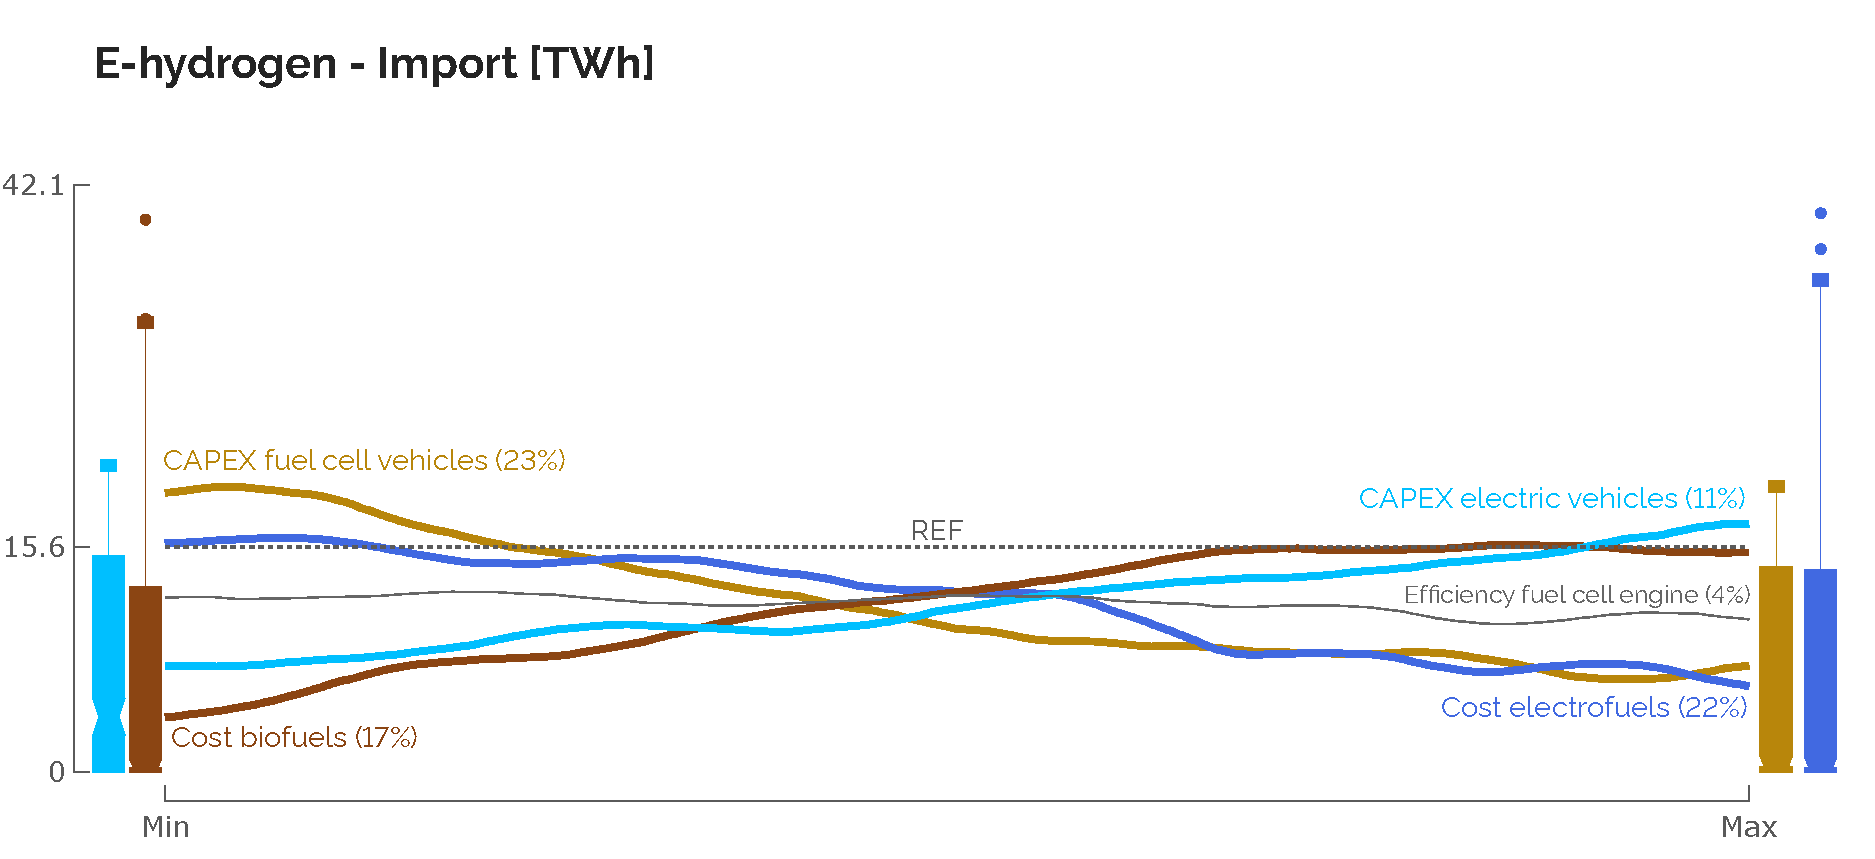
\includegraphics[width=0.8\textwidth]{UQ_H2_samples_2.pdf}
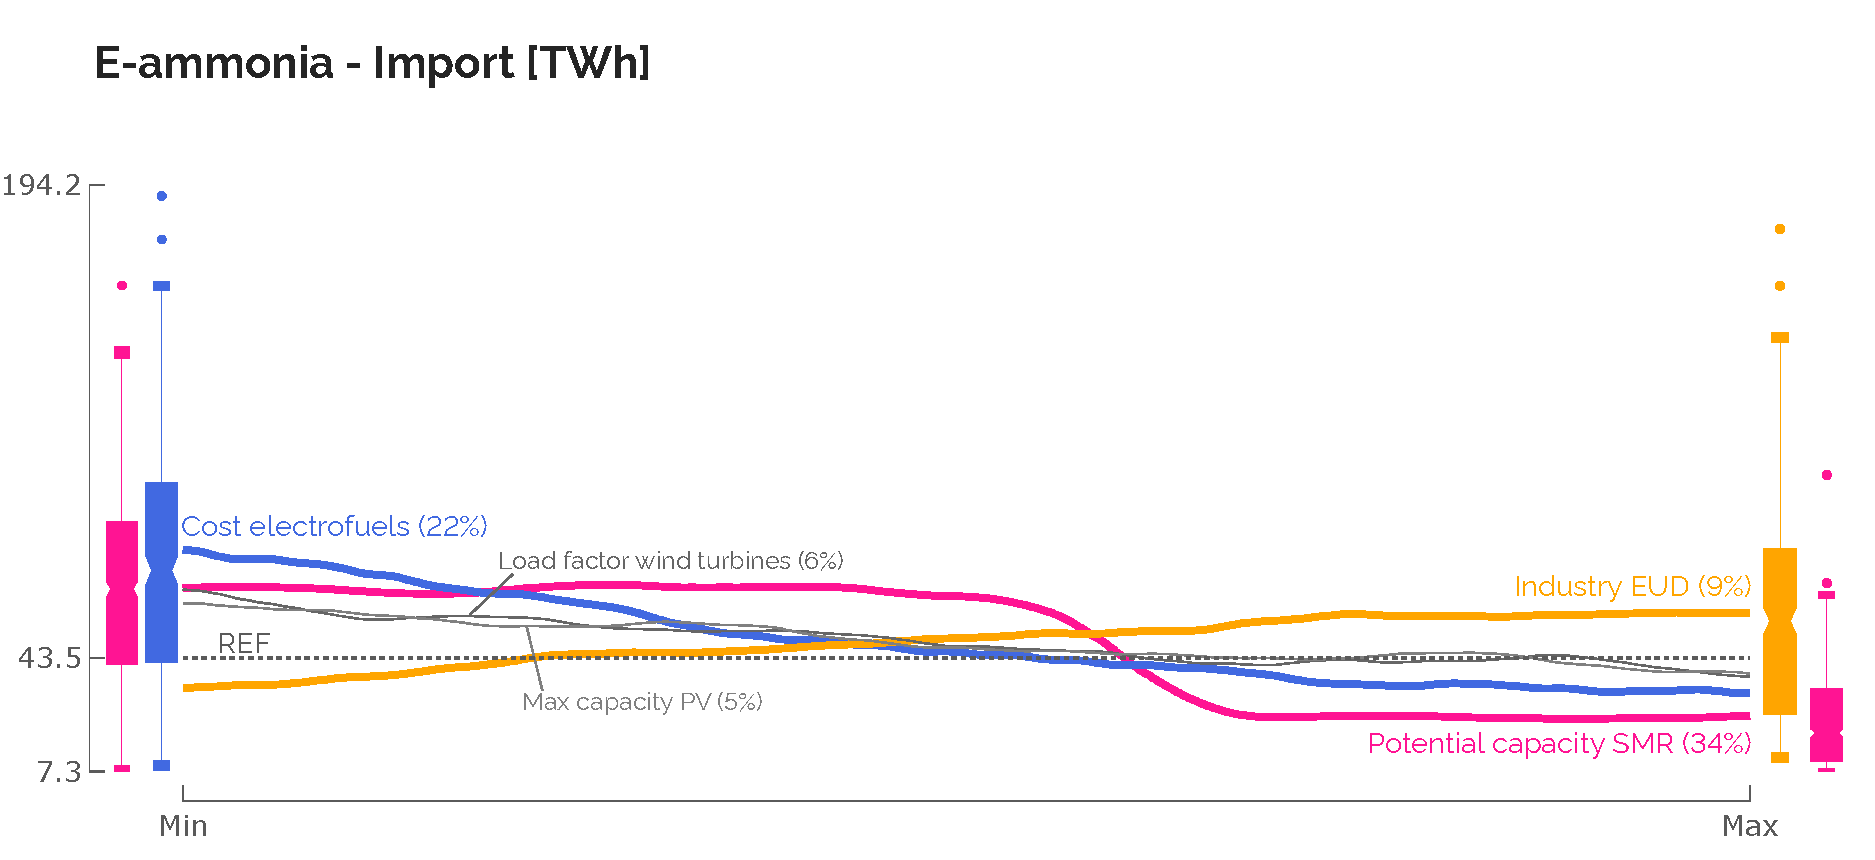
\includegraphics[width=0.8\textwidth]{UQ_Ammonia_samples_2.pdf}

\caption{Trend lines of the key parameters on the import of e-methane, e-hydrogen and e-ammonia. Around these lines, box plots point out the distribution of the output of interest for the extreme values (either bottom-15\% or top-15\%) of some parameters. The grey dashed line gives the value of the output of interest in the REF case. Part A}
\label{fig:results_uq_samples_A}
\end{figure}

\begin{figure}[htbp!]
\centering
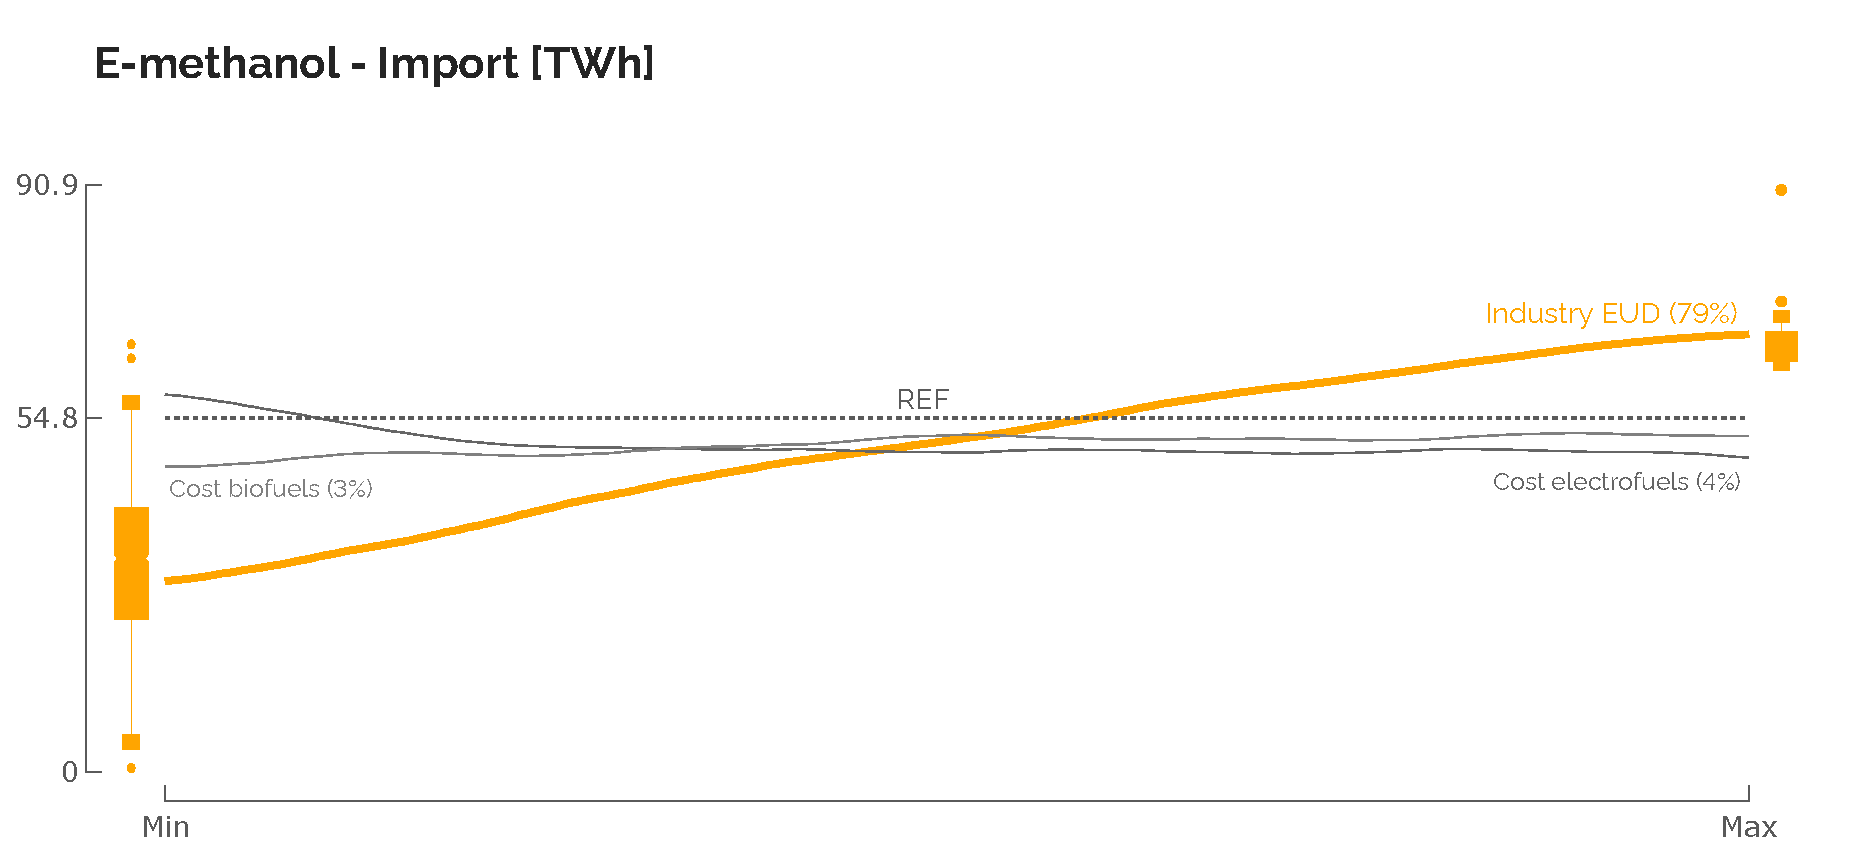
\includegraphics[width=0.8\textwidth]{UQ_Methanol_samples_2.pdf}
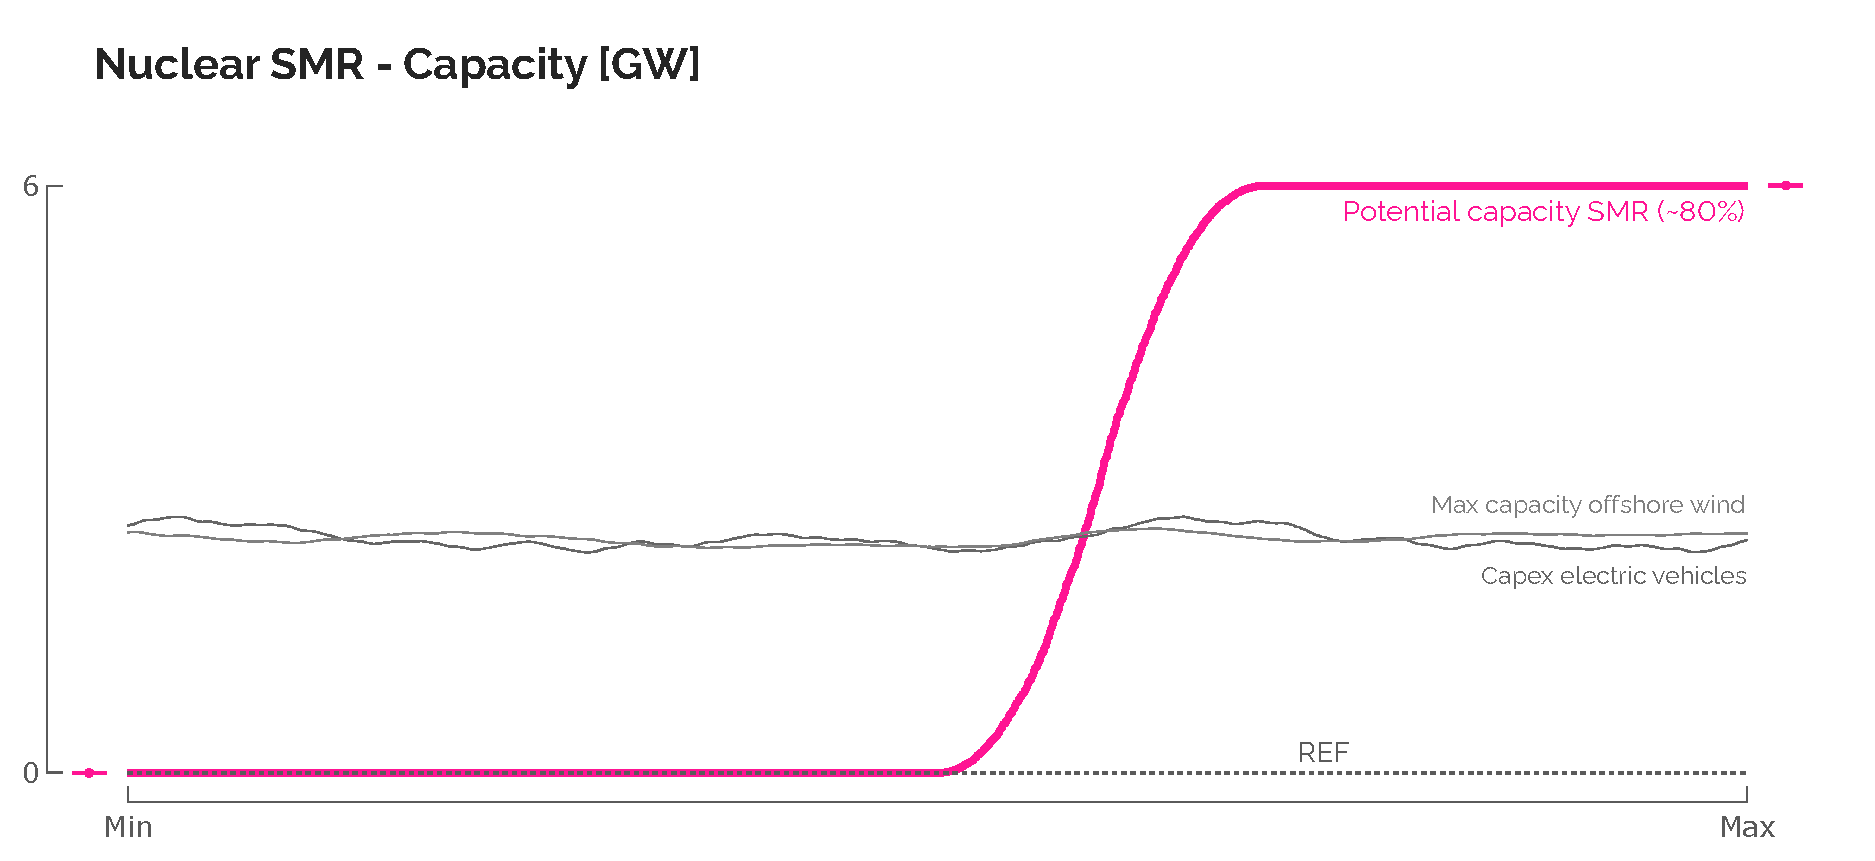
\includegraphics[width=0.8\textwidth]{UQ_SMR_samples_2.pdf}
\caption{Trend lines of the key parameters on the import of e-methanol and the installed capacity of \gls{SMR}, in 2050. Around these lines, box plots point out the distribution of the output of interest for the extreme values (either bottom-15\% or top-15\%) of some parameters. The grey dashed line gives the value of the output of interest in the REF case. Part B}
\label{fig:results_uq_samples_B}
\end{figure}

\subsection{Local renewables}
\label{subsec:atom_mol:results_uq_VRES}
In line with results given in Section \ref{sec:atom_mol:results_deter}, the \gls{GSA} shows that \gls{SMR} has negligible impact on the deployment of local \gls{VRES} (\ie \gls{PV}, onshore and offshore wind turbines). \Cref{fig:results_uq_pdf_local_ren} gives the evolution of Sobol' indices for the most impacting parameters on the deployment of \gls{PV} and offshore wind\footnote{As the installed capacities of onshore wind is totally driven by the uncertainty on its maximum potential, $f_{\mathrm{max,windon}}$, it is not represented in the figure.}. The key factor that drives the installed capacities of these two technologies is mostly their respective maximum potential, especially at the end of the transition, much more than their CAPEX. Given its higher \gls{LCOE} (\Cref{fig:LCOE}), \gls{PV} is more impacted in the short-term by the variation on the cost of purchasing electrofuels supplying e-methane (and e-ammonia to a lesser extent) \gls{CCGT}. However, this impact gets negligible by 2050.

\begin{figure}[htbp!]
\centering
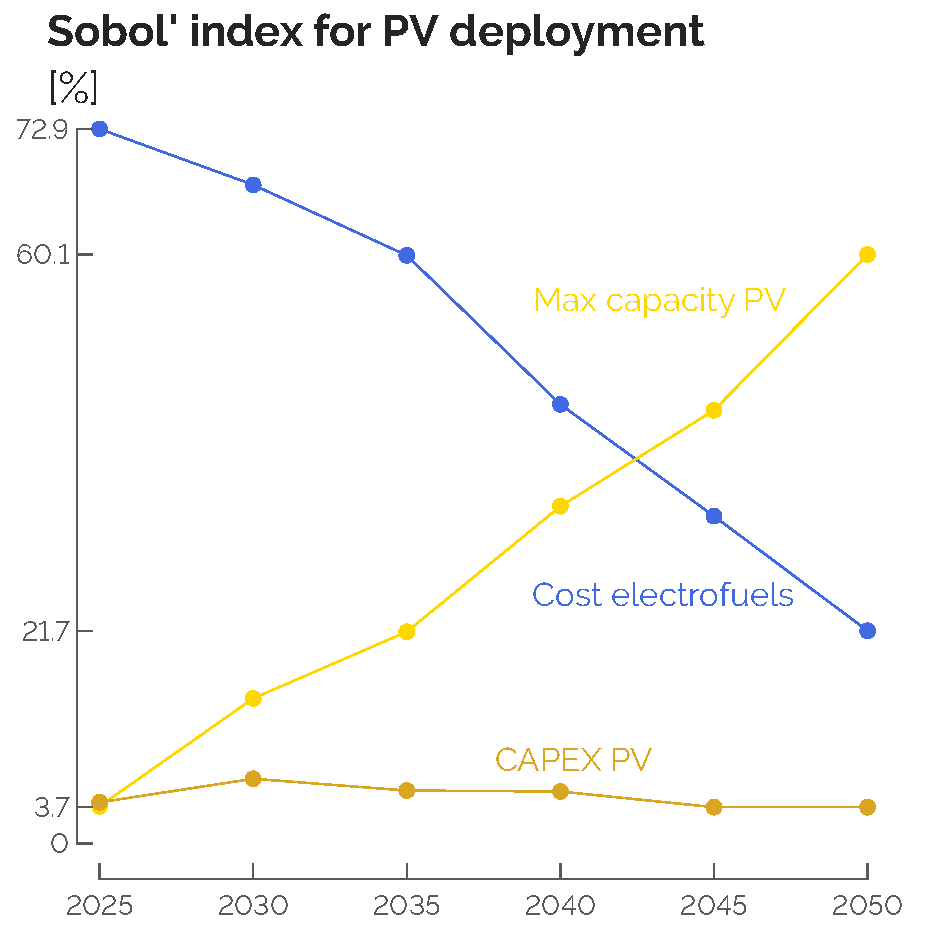
\includegraphics[width=0.49\textwidth]{Sobol_PV.pdf}
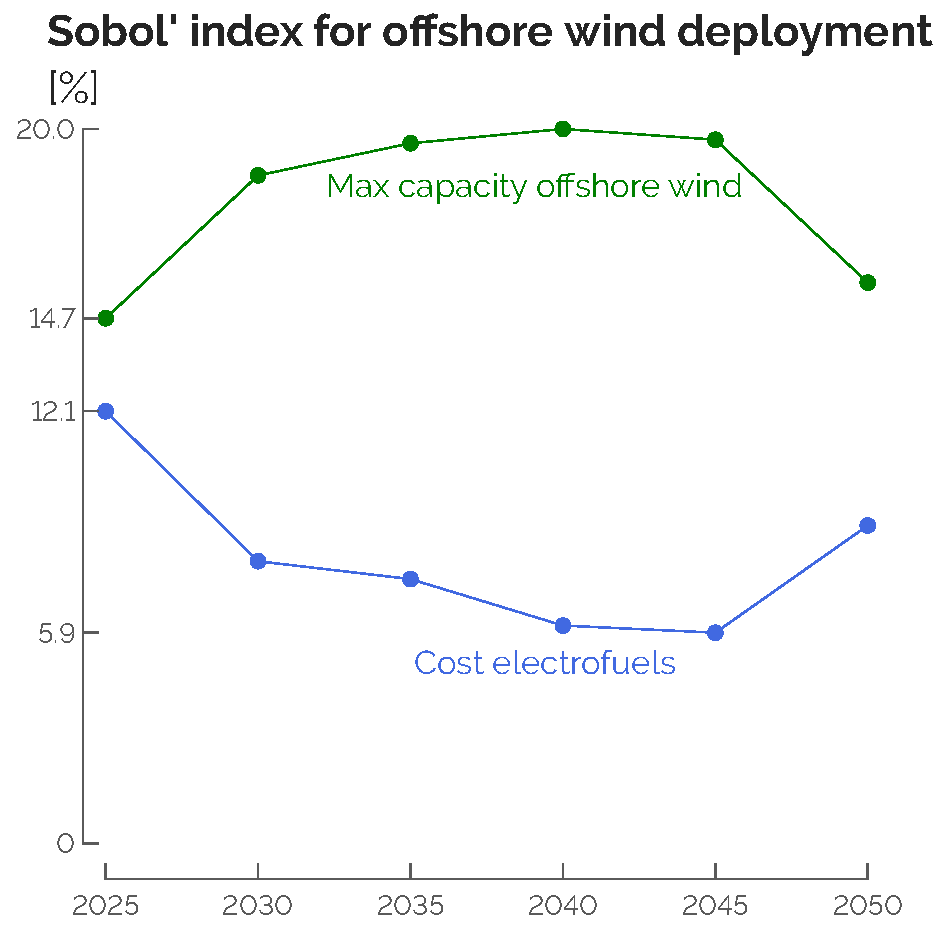
\includegraphics[width=0.49\textwidth]{Sobol_WIND_OFFSHORE.pdf}
\caption{Impacting parameters on the deployment of \gls{PV} and offshore wind over the transition. Progressively, the impact of the uncertainty on the maximum potential increases, unlike the one on the cost of purchasing electrofuels.}
\label{fig:results_uq_pdf_local_ren}
\end{figure}


\section{Discussion}
\label{sec:atom_mol:discuss}
Given its lower \gls{LCOE}, \gls{SMR} is installed as soon as available. It directly substitutes other flexible power generation units (\ie CCGT) and provides, by 2050, 44.6\,TWh, 25\% of the total electricity production. Consequently, this reduces the need to produce electricity via \gls{CHP} and allows increasing by 48\% the high-temperature heat produced by electric heaters. Besides these two sectors, the others (\ie low-temperature heat, mobility and non-energy demand) are marginally or not impacted by the integration of \gls{SMR}.

Given the ambitious \ce{CO2}-budget (\ie 30-year budget representing 10 years of the current emissions), \acrfull{GSA} highlights the biggest impact of the cost of purchasing electrofuels on the variation of the total transition cost, around 45\%. On the contrary, parameters directly related to \gls{SMR} (\ie its availability and its CAPEX) have limited impact, below 1\%. This \gls{GSA} also points out the key drivers for the import of renewable electrofuels and the installation of \gls{SMR} by 2050. Besides the cost of purchasing electrofuels (\ie the lower this cost, the bigger the imports), it shows that available \gls{SMR} would have mainly a direct impact on e-ammonia, by substituting the ammonia \gls{CCGT} that is the biggest consumer of this molecule. Indirectly, this parameter will also reduce the import of e-methane by reducing the need for gas \gls{CHP} and gas boilers. About e-hydrogen and e-methanol, their imports are impacted by the other technologies in competition in the transport sector and the industrial demand, respectively.

In conclusion, this work puts under the spotlight the ``competition'' between \gls{SMR} and imported electrofuels while both of them support to the integration of local \gls{VRES}. Betting on \gls{SMR} means letting the emissions go up at early stages of the transition (\ie \gls{LFO} still used in 2025 to produce \gls{HVC}) to end up with an overall transition and a system by 2050 that are 3.3\% and 8.8\% cheaper than in the REF case, respectively. However, given the need to import molecules at earlier stages of the transition, with or without \gls{SMR}, it seems reasonable to keep on investing in the transport and the infrastructure to support these imports. This would allow covering ourselves against the risk of eventually not having \gls{SMR} available by the end of the first half of this century. In the EnergyScope Pathway model, assuming the same technology mix as in the SMR case up to 2040 but without installing \gls{SMR} for the rest of the transition, \ie between 2040 and 2050, would require drastic (and quick) changes to still meet the \ce{CO2}-budget: around 44\,b€ of additional cumulative OPEX in purchasing electrofuels, mostly e-ammonia (+32\,TWh by 2050) and e-methane (+31\,TWh) to supply \gls{CCGT} and industrial \gls{CHP}. As a more concrete example, Fluxys, the manager of the gas network in Belgium, already presents significant investments by 2032 (\ie 1.3\,b€) to support this transition in the near future \cite{Fluxys_2023}. 

Chapters \ref{chap:chap_RL} and \ref{chap:chap_RobPol} put in practice the methodology detailed in Chapter \ref{chap:chap_methodo} to come up with a policy to get a system robust to this possibility of finally not having access to \gls{SMR}, as well as other uncertainties, especially when considering a myopic progression through the transition.